\documentclass[pdflatex,sn-mathphys]{sn-jnl}

\usepackage[T1]{fontenc}
\usepackage{graphicx}
\usepackage{mathtools}
\usepackage{newtxtext,newtxmath}
\usepackage[scaled=0.88]{inconsolata}
\linespread{1.03}
\usepackage{algorithm}
\usepackage{algpseudocode}
\usepackage{booktabs}
\usepackage{xurl}
\DeclareUrlCommand\doiurl{\def\UrlLeft{https://doi.org/}}
\DeclareUrlCommand\burl{}
\hypersetup{bookmarksdepth=2,colorlinks=true,linkcolor=black,citecolor=black,urlcolor=black}
\usepackage{multirow}

\graphicspath{{./}{figures/}}
\jyear{2026}

\theoremstyle{thmstyletwo}
\newtheorem{definition}{Definition}

\theoremstyle{thmstyletwo}
\newtheorem{remark}{Remark}

\newenvironment{botherref}{}{}

\raggedbottom

\begin{document}

\title[EVM-Guard: Bytecode Reentrancy Triage]{EVM-Guard: Bytecode-Only Reentrancy Triage for Solidity 0.4--0.5 with Sandbox Witness Replay}

\author{\fnm{Devarsh} \sur{Patel}}\email{devarsh.patel2024@vitstudent.ac.in}

\affil{\orgdiv{School of Computer Science and Engineering}, \orgname{Vellore Institute of Technology}, \orgaddress{\city{Vellore}, \postcode{632014}, \state{Tamil Nadu}, \country{India}}}

\abstract{
Reentrancy remains one of the most frequently reported causes of loss in Ethereum contracts, and many deployed contracts are available only as bytecode. This paper describes the design and evaluation of \textbf{EVM-Guard}, a bytecode-only triage tool for reentrancy in contracts compiled with Solidity 0.4--0.5. Engine v5 builds a control-flow graph with an abstract-stack dataflow and flags an external call that is followed on some path by a storage write without an intervening mutex; calls that forward only the 2300-gas stipend are excluded, and each candidate is replayed in a \texttt{py-evm} sandbox. Engine v6 adds return-site tracking, a Z3 path-feasibility check under an unprivileged-attacker model, and a replay seeded with the solver's witness. On SmartBugs-curated, v5 reached 93.5\% reentrancy recall at 80.6\% precision (95\% CI 64.0--91.8); this figure is post hoc. When Slither was restricted to its \texttt{reentrancy-eth} and \texttt{reentrancy-no-eth} detectors, no significant difference in false positives was found (McNemar $p = 0.69$), whereas the bytecode analysers EVMLiSA and eThor produced significantly more false positives than v5 on every corpus on which they were run ($p \le 1.3 \times 10^{-4}$). In the two most recent pre-registered synthetic tests, with 210 contracts each, both engines achieved 100\% recall and precision on Solidity 0.5.12, and v6 detected all 30 injected reentrancies on Solidity 0.8.20, none of which v5 detected. On SolidiFI and a labelled benchmark that had not been used in its development, however, v6 produced more false positives than v5 ($p = 9.5 \times 10^{-7}$ and $0.021$), and v5 was therefore retained as the default engine. Of 3,214 deployed Solidity 0.4--0.5 contracts holding 45,217 ether, v5 flagged 522, with a median analysis time of 0.48\,s per contract. A blind manual review of 120 flagged contracts identified one exploitable contract, which corresponds to a precision of 1.6\% for v5 (95\% CI 0.04--8.7); on the same contracts, v5 produced fewer false positives than strict Slither ($p = 0.021$). Most flags on deployed code concerned calls to fixed or trusted addresses, which suggests that the output of EVM-Guard on such code is best treated as a list for manual review. Denial-of-service and arithmetic hazards are reported as exploratory results only.
}

\keywords{Smart Contract Security, Reentrancy, EVM Bytecode, Static Analysis, Path Feasibility, Z3, McNemar Test}

\maketitle

%% ===========================================================================
\section{Introduction}\label{sec:intro}

\subsection{Motivation}\label{sec:intro:motivation}
Transactions on Ethereum cannot be reversed, and deployed bytecode cannot be patched in place. A contract that makes an external call before it has updated its own storage can therefore be re-entered and drained before the update takes effect. Surveys of attacks on deployed contracts have identified reentrancy, oracle manipulation and arithmetic errors as recurring sources of loss~\cite{zhou2023sok,chen2020survey}, and transaction ordering can make such attacks easier to carry out~\cite{daian2020flash}. Since the source code of many deployed contracts has not been published, there is a need for analysers that work on runtime bytecode alone.

\subsection{Existing Analysis Approaches}\label{sec:intro:approaches}
\begin{enumerate}
    \item \textbf{Static analysis over intermediate representations.} Source-level analysers such as Slither~\cite{feist2019slither} translate the compiler's abstract syntax tree into an intermediate representation, so they cannot be applied when only bytecode is available. Bytecode analysers such as Securify~\cite{tsankov2018securify} encode basic blocks as relational facts that are evaluated with Souffl{\'e}~\cite{scholz2016souffle}, but they abstract over stack depth and gas arithmetic, and evaluations of such tools have reported false-positive rates above 50\%~\cite{durieux2020empirical,ghaleb2020how}.
    \item \textbf{Symbolic execution.} Symbolic execution frameworks, including Mythril\footnote{\url{https://github.com/Consensys/mythril}; version 0.24.8 was used.}, Manticore~\cite{mossberg2019manticore} and Oyente~\cite{luu2016making}, check path feasibility by passing path conditions to the Z3 solver~\cite{de2008z3}. On non-trivial contracts, loops that depend on storage and hashing instructions cause the number of paths to grow rapidly. In the evaluation reported here, Mythril timed out on 25.9\% of the SmartBugs files and on 77.0\% of the SolidiFI files. Exploit generators such as teEther~\cite{krupp2018teether} and fuzzers such as Echidna~\cite{grieco2020echidna} and ConFuzzius~\cite{torres2021confuzzius} produce concrete inputs, although several of them require properties or a test harness to be written by hand.
    \item \textbf{Property testing and deductive verification.} hevm~\cite{dxo2024hevm} executes bytecode symbolically in order to check assertions written by the developer, and VerX~\cite{permenev2020verx} and KEVM~\cite{hildenbrandt2018kevm} verify temporal properties against formal specifications. These tools give strong guarantees for the properties that are stated, but a specification has to be written for every contract.
\end{enumerate}
EVM-Guard works on compiled runtime bytecode and needs neither annotations nor a test harness. Engine v5 evaluates fixed dataflow patterns over the recovered control-flow graph (CFG) and follows CFG reachability without solving path conditions. Engine v6 retains a v5 candidate only if Z3 cannot refute both a path to the candidate and a re-entrant run from the state at the call (Section~\ref{sec:arch:v6}). Neither engine proves that a hazard is absent (Section~\ref{sec:arch:scope}).

\subsection{Research Questions}\label{sec:intro:rqs}
This study sought to answer the following research questions:
\begin{itemize}
    \item \textbf{RQ1 (Detection precision):} Can CFG dataflow tracking within a function and the recognition of storage-slot mutexes reduce reentrancy false positives in comparison with source-level tools, while recall on benchmark suites remains high?
    \item \textbf{RQ2 (Replay):} To what extent can sandbox replay confirm static warnings without false alarms, and how much recall is lost when only confirmed findings are counted?
    \item \textbf{RQ3 (Generalisation):} How does precision on the benchmarks used during development compare with precision on held-out synthetic corpora, including one compiled with Solidity 0.8?
    \item \textbf{RQ4 (Deployed contracts):} How many deployed Solidity 0.4--0.5 contracts does EVM-Guard flag, at what cost, and how many of the flags prove exploitable on manual review?
\end{itemize}

\subsection{Contributions}\label{sec:intro:contrib}
The main contributions of this paper are as follows.
\begin{enumerate}
    \item \textbf{Hazard specifications and a reentrancy dataflow check.} Bit-vector specifications over $\mathcal{BV}_{256}$ are stated for six hazard classes, including read-only reentrancy (Section~\ref{sec:formal_framework}), together with the CFG dataflow checks and Z3 parameter templates that EVM-Guard implements (Table~\ref{tab:impl}). The checks approximate these specifications and are not proved to decide them (Section~\ref{sec:arch:scope}). Calls restricted to the 2300-gas stipend are excluded from the reentrancy check.
    \item \textbf{A bytecode analyser with sandbox replay.} EVM-Guard recovers basic-block CFGs from disassembled bytecode, computes an abstract-stack fixpoint, and replays candidate transactions in a \texttt{py-evm} sandbox, where a finding is confirmed only if a post-state criterion on balances or storage is met (Section~\ref{sec:arch}).
    \item \textbf{A path-feasibility engine.} Engine v6 adds return-site tracking, a Z3 path search under an unprivileged-attacker model that classifies each finding as same-function, cross-function or read-only reentrancy, and witness-seeded replay (Section~\ref{sec:arch:v6}). It was frozen before it was evaluated, and its results are reported alongside those of v5 on the same files (Section~\ref{sec:v6}).
    \item \textbf{Benchmark evaluation with paired tests.} Results are reported for SmartBugs-curated (143 files), SolidiFI (400 files), a labelled benchmark (389 files) and a series of pre-registered synthetic tests, against Slither, Mythril, EVMLiSA, eThor and the static stage of Sailfish, with exact McNemar tests on the same files. Figures obtained after the engine had been revised on a corpus are marked as post hoc (Sections~\ref{sec:results} and~\ref{sec:baselines}).
    \item \textbf{A study of deployed contracts.} Both engines were run on 3,214 deployed Solidity 0.4--0.5 contracts that hold ether, and a blind random sample of 120 flagged contracts was reviewed by hand (Section~\ref{sec:v6:mainnet}).
\end{enumerate}

%% ===========================================================================
\section{Related Work and Hazard Classes}\label{sec:gaps}

Table~\ref{tab:paradigm_comparison} lists the tools that are closest to EVM-Guard, together with the input that each of them requires. Tool speeds are not included in the table, because the published figures were not obtained under a common protocol; timing is compared only for the runs reported in this paper (Section~\ref{sec:results:runtime}).

\begin{table*}[t]
\centering
\small
\caption{Qualitative comparison of EVM analysis tools. ``User spec.'' means the user must write assertions, harnesses or formal specifications before the tool can check a property.}
\label{tab:paradigm_comparison}
\resizebox{\textwidth}{!}{%
\begin{tabular}{@{}llllc@{}}
\toprule
\textbf{Tool} & \textbf{Technique} & \textbf{Input} & \textbf{Requires} & \textbf{User spec.} \\
\midrule
Slither~\cite{feist2019slither} & Pattern and dataflow rules on an IR & Source & Solidity source & No \\
Securify~\cite{tsankov2018securify} & Datalog compliance patterns & Source or bytecode & solc for source; bytecode accepted & No \\
Mythril & Symbolic execution with SMT & Source or bytecode & Solidity or bytecode & No \\
Manticore~\cite{mossberg2019manticore} & Symbolic execution & Source or bytecode & Solidity or bytecode & Optional \\
Echidna~\cite{grieco2020echidna} & Property-based fuzzing & Source & Properties to test & Yes \\
ConFuzzius~\cite{torres2021confuzzius} & Hybrid fuzzing with data dependencies & Source, or ABI of a deployed contract & Solidity source, or ABI and a chain node & No \\
VerX~\cite{permenev2020verx} & Deductive verification & Source & Formal specification & Yes \\
hevm~\cite{dxo2024hevm} & Symbolic execution of assertions & Bytecode & Test harness & Yes \\
Gigahorse~\cite{grech2019gigahorse} & Decompilation to a register IR, Datalog clients & Bytecode & Bytecode only & No \\
eThor~\cite{schneidewind2020ethor} & Sound static analysis by Horn-clause abstraction & Bytecode & Bytecode only & No \\
EVMLiSA~\cite{arceri2026evmlisa} & Abstract interpretation (LiSA) with a reentrancy checker & Bytecode & Bytecode only & No \\
Sailfish~\cite{bose2022sailfish} & Storage dependency graph with symbolic refinement & Source & Solidity source & No \\
\textbf{EVM-Guard} & CFG dataflow (v5); Z3 path feasibility and witness replay (v6) & Runtime bytecode & Bytecode only & No \\
\bottomrule
\end{tabular}%
}
\end{table*}

\paragraph{Bytecode reentrancy analysers.} eThor~\cite{schneidewind2020ethor} abstracts EVM bytecode into Horn clauses and attempts to prove single-entrancy, a property that excludes reentrancy. Since the analysis is sound with respect to its semantics, a contract is reported as insecure whenever the property cannot be proved. EVMLiSA~\cite{arceri2026evmlisa} constructs a sound CFG of the bytecode by abstract interpretation of the stack in the LiSA framework and applies a reentrancy checker to it. Gigahorse~\cite{grech2019gigahorse} decompiles bytecode into a register-based intermediate representation on which Datalog clients are run. Sailfish~\cite{bose2022sailfish}, in contrast, operates on source code: a storage dependency graph proposes reentrancy and transaction-ordering candidates, which a symbolic verifier then refines. EVM-Guard is compared with eThor, EVMLiSA and Sailfish in Section~\ref{sec:baselines}. Gigahorse is not used as a baseline, since it is a decompilation framework and has no reentrancy client of its own.

\subsection{Positioning against hevm}\label{sec:gaps:hevm}
hevm~\cite{dxo2024hevm} checks assertions that a developer has written into a test harness, typically a Foundry property test, and explores the paths of the contract under their path conditions; a counterexample produced by hevm is therefore tied to the semantics of the contract. EVM-Guard, by contrast, needs no harness or assertion and applies a fixed set of checks to any runtime bytecode. The price of this generality is lower precision. Because the checks only approximate the specifications of Section~\ref{sec:formal_framework}, a finding indicates a hazard and is not a counterexample to a stated property. The two kinds of tool may therefore be regarded as complementary: EVM-Guard can be used to triage unannotated bytecode, and a property-testing tool can then confirm a suspected hazard once the property has been written.

\subsection{Hazard Classes}\label{sec:gaps:taxonomy}
EVM-Guard targets six hazard classes, which are mapped to SWC identifiers in Table~\ref{tab:gap_taxonomy}. The specifications were written for this study; the citations refer to earlier work on the same class.

\begin{table*}[t]
\centering
\small
\caption{Hazard classes targeted by EVM-Guard and the corresponding specification (Section~\ref{sec:math:invariants}).}
\label{tab:gap_taxonomy}
\resizebox{\textwidth}{!}{%
\begin{tabular}{@{}lcp{5.6cm}p{6.8cm}@{}}
\toprule
\textbf{Class} & \textbf{SWC} & \textbf{Hazard} & \textbf{Specification} \\
\midrule
A & SWC-107 & A callee observes or changes state before the caller settles its own storage~\cite{rodler2021sereum,grossman2018online}. & $\Phi_{\mathrm{RO}}$ (Def.~\ref{prop:ro}) \\
B & SWC-101 & Fixed-point division truncation that discards remainders. & $\Phi_{\mathrm{Prec}}$ (Def.~\ref{prop:prec}) \\
C & SWC-124 & Proxy and implementation assigning one storage slot to variables of different widths. & $\Phi_{\mathrm{Slot}}$ (Def.~\ref{prop:proxy}) \\
D & SWC-128 & Loops over user-growable storage arrays that exceed a gas limit~\cite{grech2018madmax}. & $\Phi_{\mathrm{DoS}}$ (Def.~\ref{prop:dos}) \\
E & Non-SWC & Lending logic that reads AMM spot reserves as a price oracle~\cite{zhou2023sok}. & $\Phi_{\mathrm{Flash}}$ (Def.~\ref{prop:flash}) \\
F & SWC-112 & \texttt{DELEGATECALL} target influenced by calldata. & $\Phi_{\mathrm{Taint}}$ (Def.~\ref{prop:taint}) \\
\bottomrule
\end{tabular}%
}
\end{table*}

\paragraph{Class A: reentrancy (SWC-107).} A contract makes an external call before it has updated its own storage, and the callee re-enters it. In read-only reentrancy, a view function returns unsettled state to a third contract while the call is in progress. The check in EVM-Guard follows CFG edges from an external call to a later storage write in the same function and tests whether a mutex intervenes. Engine v5 does not distinguish between these variants, whereas engine v6 records whether the re-entrant run reaches the same call, a stale read in another function, or a stale read in a function that writes nothing (Definition~\ref{def:reentrancy}).

\paragraph{Class B: division truncation (SWC-101).} Integer division $\lfloor x/y \rfloor$ discards the remainder, and division before multiplication increases the loss. SWC-101 also covers integer overflow and underflow, but EVM-Guard targets truncation only, a distinction that matters for the SmartBugs arithmetic category (Section~\ref{sec:results:arith}).

\paragraph{Class C: storage-slot collision (SWC-124).} Upgradeable contracts execute implementation logic in the storage of the proxy through \texttt{DELEGATECALL}, and a mismatch between the two storage layouts can overwrite critical variables such as the owner.

\paragraph{Class D: loop gas exhaustion (SWC-128).} A loop over a dynamic storage array that any user can extend may grow until the call no longer fits within the gas limit.

\paragraph{Class E: spot-price oracle manipulation.} A flash loan can move the spot reserves of an automated market maker within a single transaction. The SWC registry has no identifier for this class (SWC-114 denotes transaction order dependence), and these findings are therefore referred to as Class~E. The output files of the tool record them under the internal label \texttt{SWC-114}, which does not refer to the registry entry. SmartBugs has no corresponding category, so these findings are reported but not scored.

\paragraph{Class F: delegatecall taint (SWC-112).} If calldata determines the target of a \texttt{DELEGATECALL}, an attacker can execute arbitrary code in the storage context of the caller.

%% ===========================================================================
\section{Hazard Specifications over \texorpdfstring{$\mathcal{BV}_{256}$}{BV256}}\label{sec:formal_framework}

The definitions in this section are specifications; they do not describe what the implementation proves. Definitions~\ref{def:attacker}--\ref{def:pattern} state the reentrancy property that EVM-Guard targets and the pattern that its check reports, and Section~\ref{sec:arch:scope} and Table~\ref{tab:impl} describe how each engine approximates them. Definitions~\ref{prop:proxy}--\ref{prop:taint} specify the other hazard classes, for which results are reported but no claims are made.

\subsection{Notation}\label{sec:math:state}
An execution frame is $\mathcal{S} \triangleq \langle \mathbf{\sigma}, \mathbf{\tau}, \mathbf{\mu}, \mathbf{\iota} \rangle$, where $\mathbf{\sigma}: \mathcal{BV}_{256} \to \mathcal{BV}_{256}$ is persistent storage, $\mathbf{\tau}$ is EIP-1153 transient storage, $\mathbf{\mu}$ is the machine state (stack, memory, program counter, gas), and $\mathbf{\iota}$ is the transaction context, including the caller $\iota.\mathit{caller}$. Words are elements of $\mathcal{BV}_{256}$ with arithmetic modulo $2^{256}$. For $v \neq 0$, $\mathrm{UDiv}(u, v) \triangleq \lfloor u / v \rfloor$ and $\mathrm{URem}(u, v) \triangleq u - v \cdot \mathrm{UDiv}(u, v)$, with $\mathrm{UDiv}(u, 0) = \mathrm{URem}(u, 0) = 0$, in agreement with the \texttt{DIV} and \texttt{MOD} opcodes in formal operational semantics of the EVM~\cite{grishchenko2018semantic,hildenbrandt2018kevm}. The condition
\begin{equation}
    \mathrm{NoMulOverflow}(u, v) \equiv (v = 0) \lor \big(\mathrm{UDiv}(u \cdot v, v) = u\big)
\end{equation}
expresses that the wrapped product $u \cdot v$ equals the mathematical product. For a contract $C$, a public function $f$ is the code reached from the dispatcher entry of one selector. A run $\sigma \xrightarrow{f,\,d,\,a} \sigma'$ executes $f$ with calldata $d$ and caller $a$ from storage $\sigma$ and ends in $\sigma'$ without reverting. Inside a run, an external call site $c$ is a \texttt{CALL} or \texttt{CALLCODE} instruction; $\sigma_c$ is the storage when $c$ executes, $t_c$ the callee address and $g_c$ the forwarded gas.

\subsection{Reentrancy}\label{sec:math:reentrancy}

\begin{definition}[Unprivileged attacker]\label{def:attacker}
Let $K(C)$ be the 20-byte constants in the bytecode of $C$, and let $\mathrm{Fixed}(\sigma)$ be the addresses held, at any byte offset, in storage slots of $\sigma$ whose index is a constant of the bytecode. A slot is \emph{settable} if some public function writes it with a value derived from the caller, or from calldata on a path not guarded by a caller check. An address $A$ is an unprivileged attacker for $C$ in state $\sigma$ if
\begin{equation}
    \mathrm{Unpriv}(A, \sigma) \equiv A \notin K(C) \;\land\; A \notin \mathrm{Fixed}^{\neg\mathrm{set}}(\sigma),
\end{equation}
where $\mathrm{Fixed}^{\neg\mathrm{set}}$ ranges over the slots that are not settable. The attacker sends the transaction, controls the code at $A$, and therefore controls what happens when $A$ is called.
\end{definition}

\begin{definition}[Reentrancy hazard]\label{def:reentrancy}
Contract $C$ has a reentrancy hazard at call site $c$ of public function $f$ if there are a state $\sigma$, calldata $d$ and an address $A$ with $\mathrm{Unpriv}(A, \sigma)$ such that a run $\sigma \xrightarrow{f,\,d,\,A}$ reaches $c$ with
\begin{equation}
    t_c = A \;\land\; g_c > 2300 \;\land\; \exists w \text{ after } c \text{ in } f: w \text{ writes slot } k,
\end{equation}
and a re-entrant run $\sigma_c \xrightarrow{g,\,d',\,A}$ started from the storage at the call reaches either (i) $c$ again, with $g = f$ (\emph{same-function} reentrancy), or (ii) a read of slot $k$, with $g \neq f$ (\emph{cross-function} reentrancy; \emph{read-only} if $g$ writes no storage and makes no call). The write $w$ makes the re-entrant run observe a state that $f$ has not settled.
\end{definition}

Definition~\ref{def:reentrancy} is a single-transaction property relative to an arbitrary starting state $\sigma$. It requires neither that $\sigma$ be reachable from deployment nor that re-entry be profitable. Section~\ref{sec:arch:scope} records which parts of it each engine checks, and the labelling rubric of the study of deployed contracts (Section~\ref{sec:v6:mainnet}) adds the requirement of profit.

\begin{definition}[Reentrancy pattern]\label{def:pattern}
Let $R(f)$ be the blocks reachable from the entry of $f$ without entering another function's entry. Call site $c$ in $R(f)$ matches the reentrancy pattern if the abstract gas bound of $c$ exceeds 2300, some \texttt{SSTORE} $w$ in $R(f)$ is reachable from $c$ along CFG edges inside $R(f)$, and no mutex (a dominating write before $c$, a branch on the written slot before $c$, and a reset reachable after $c$) guards $c$.
\end{definition}

Engine v5 reports every match of Definition~\ref{def:pattern}. Engine v6 reports a match only if Z3 does not refute the two runs of Definition~\ref{def:reentrancy} under the attacker of Definition~\ref{def:attacker} (Section~\ref{sec:arch:v6}).

\begin{remark}[What a rejection means]\label{rem:rejection}
The symbolic model of engine v6 replaces every value that it cannot compute exactly (environment reads, results of external calls, hashes and unaligned memory) with an unconstrained symbol, so that every concrete run along a modelled path satisfies its path condition. If Z3 reports the path condition as unsatisfiable, no run can follow that path. This argument holds only for the modelled operations and for the bounded set of paths explored; it concerns the implementation and is not a machine-checked proof. A search that reaches one of its limits rejects nothing.
\end{remark}

\begin{definition}[Read-only reentrancy ($\Phi_{\mathrm{RO}}$)]\label{prop:ro}
Let $\mathbf{\sigma}_{\mathrm{transient}}$ be the storage state during an external call and $\mathbf{\sigma}_{\mathrm{settled}}$ the state after the call. A contract violates read-only reentrancy safety if some public view function $f_{\mathrm{view}}$ returns different values in the two states:
\begin{equation}
    \Phi_{\mathrm{RO}} \equiv \mathrm{InExternalCall}(\mathbf{\iota}) \land \Big( f_{\mathrm{view}}(\mathbf{\sigma}_{\mathrm{transient}}) \neq f_{\mathrm{view}}(\mathbf{\sigma}_{\mathrm{settled}}) \Big)
\end{equation}
This is the read-only case (ii) of Definition~\ref{def:reentrancy}, stated in terms of the result of the view function.
\end{definition}

\subsection{Other hazard classes}\label{sec:math:invariants}

\begin{definition}[Proxy storage-slot collision ($\Phi_{\mathrm{Slot}}$)]\label{prop:proxy}
Let implementations $C_1$ and $C_2$ have slot assignments $\mathcal{L}_1, \mathcal{L}_2$ and types $\mathcal{T}_1, \mathcal{T}_2$. A collision exists if two variables mapped to the same slot have different bit-widths:
\begin{equation}
\begin{aligned}
    \Phi_{\mathrm{Slot}} \equiv \exists v_1 \in \mathrm{Var}(C_1), v_2 \in \mathrm{Var}(C_2) : {} & \big( \mathcal{L}_1(v_1) = \mathcal{L}_2(v_2) \big) \land {} \\
    & \big( \mathrm{BitWidth}(\mathcal{T}_1(v_1)) \neq \mathrm{BitWidth}(\mathcal{T}_2(v_2)) \big)
\end{aligned}
\end{equation}
\end{definition}

\begin{definition}[Fixed-point truncation ($\Phi_{\mathrm{Prec}}$)]\label{prop:prec}
Let fixed-point division with scale $10^k$ ($k \in \{6, 18\}$) compute $\mathrm{UDiv}(x \cdot 10^k, y)$. A truncation hazard exists if
\begin{equation}
\begin{aligned}
    \Phi_{\mathrm{Prec}} \equiv \exists x, y \in \mathcal{BV}_{256} : \quad & (y > 0) \land \mathrm{NoMulOverflow}(x, 10^k) \land {} \\
    & (\mathrm{URem}(x \cdot 10^k, y) \neq 0) \land {} \\
    & \left( \mathrm{UDiv}(\mathrm{URem}(x \cdot 10^k, y)\cdot 10^k, y) > 0 \right)
\end{aligned}
\end{equation}
This predicate holds for almost any division that leaves a non-zero remainder. It is therefore a necessary but not a sufficient condition for a truncation hazard, which is consistent with the high arithmetic false-positive rate reported in Section~\ref{sec:results:arith}.
\end{definition}

\begin{definition}[Loop gas exhaustion ($\Phi_{\mathrm{DoS}}$)]\label{prop:dos}
Out-of-gas and resource-exhaustion hazards have been studied extensively for the EVM~\cite{grech2018madmax,albert2020gasol,perez2020broken}. Let $N$ be the length of a dynamic storage array iterated by a loop, $C_0$ the base call cost and $c_{\mathrm{step}}$ the per-iteration cost, so $C_{\mathrm{total}}(N) = C_0 + N \cdot c_{\mathrm{step}}$. For a gas threshold $G$, a denial-of-service hazard exists if an unprivileged function can grow $N$ without a static bound and
\begin{equation}
    \Phi_{\mathrm{DoS}}(G) \equiv \mathrm{IsMutatorPublic}(f_{\mathrm{mut}}) \land \neg \mathrm{HasStaticBound}(N) \land \big( C_0 + N \cdot c_{\mathrm{step}} > G \big)
\end{equation}
The static Z3 template sets $G_{\mathrm{block}} = 30 \times 10^6$, the gas limit of the genesis block of the sandbox, with $C_0 = 21{,}000$ and $c_{\mathrm{step}} = 5{,}000$. A scaled threshold, $G_{\mathrm{sandbox}} = 1.5 \times 10^6$, is used only by the replay oracle (Section~\ref{sec:arch:oracle}), which limits each replayed transaction to $G_{\mathrm{sandbox}}$ gas and confirms a finding when the call exhausts that limit. A confirmation therefore shows unbounded growth at a reduced scale, not the exhaustion of a full block.
\end{definition}

\begin{definition}[Spot-price oracle manipulation ($\Phi_{\mathrm{Flash}}$)]\label{prop:flash}
Let an AMM hold reserves $x, y$ with fee $\phi \in [0,1)$, and let the post-swap spot price be $P_1(\Delta x) = \frac{x + \Delta x (1-\phi)}{y - \Delta y}$. If a lending protocol prices collateral $C$ and debt $D$ at the spot price $P_0 = x/y$, a position solvent at $P_0$ can be pushed below the solvency threshold $H_{\mathrm{min}}$ when
\begin{equation}
\begin{aligned}
    \Phi_{\mathrm{Flash}} \equiv \exists \Delta x : {} & (0 < \Delta x \le \Lambda_{\mathrm{max}}) \land \left( \tfrac{C \cdot P_0}{D} \ge H_{\mathrm{min}} \right) \land {} \\
    & \left( \tfrac{C \cdot P_1(\Delta x)}{D} < H_{\mathrm{min}} \right)
\end{aligned}
\end{equation}
\end{definition}

\begin{definition}[Delegatecall target taint ($\Phi_{\mathrm{Taint}}$)]\label{prop:taint}
Let $T_{\mathrm{target}} \in \mathcal{BV}_{160}$ be the \texttt{DELEGATECALL} target operand and $\mathrm{AuthorizedTarget}$ the set of permitted callees. On a path $\pi$ with path condition $\mathrm{PC}(\pi)$, the call is hijackable if
\begin{equation}
\begin{aligned}
    \Phi_{\mathrm{Taint}} \equiv \exists \mathbf{d}, A_{\mathrm{attacker}} : {} & \mathrm{PC}(\pi) \land (T_{\mathrm{target}}(\mathbf{d}) = A_{\mathrm{attacker}}) \land {} \\
    & (A_{\mathrm{attacker}} \notin \mathrm{AuthorizedTarget})
\end{aligned}
\end{equation}
\end{definition}

\begin{remark}[Unimplemented specification]
The interpreter of EVM-Guard does not model \texttt{TSTORE} or \texttt{TLOAD}, and it therefore has no check for divergence of transient-storage locks. Since no contract in the evaluation corpora uses EIP-1153, this omission does not affect the results.
\end{remark}

%% ===========================================================================
\section{System Architecture and Implementation}\label{sec:arch}

\begin{figure*}[t]
\centering
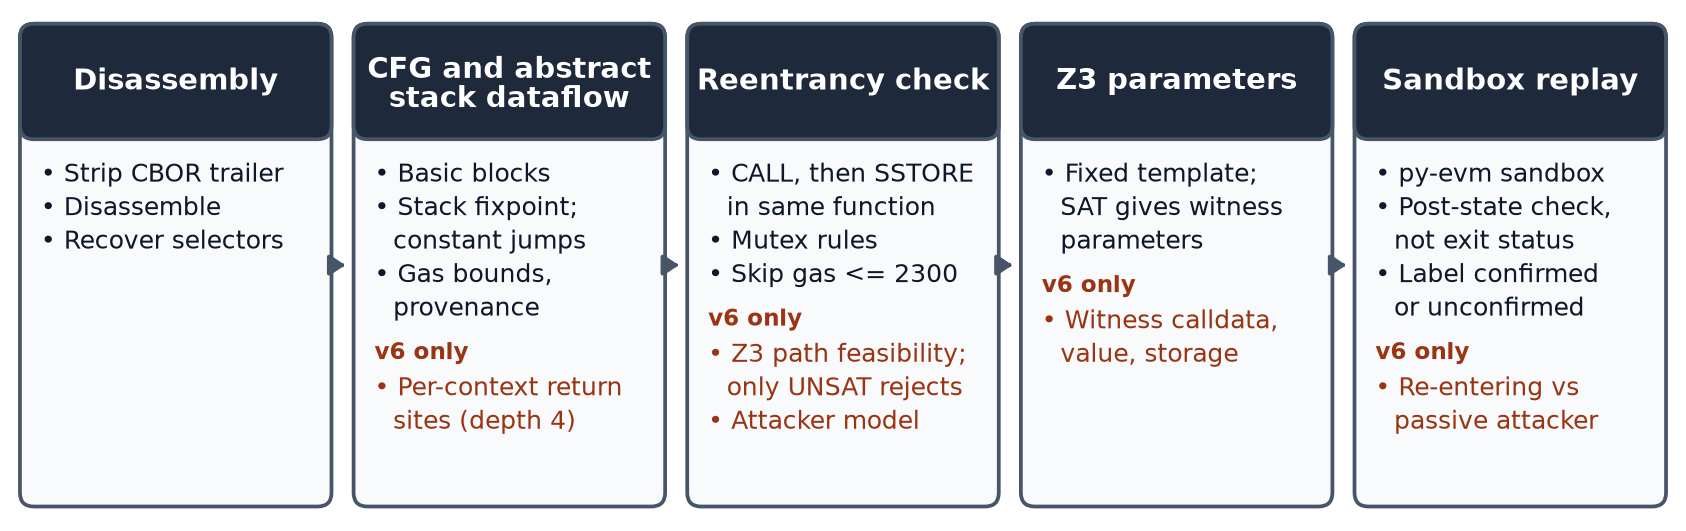
\includegraphics[width=\textwidth]{fig_pipeline_architecture.png}
\caption{The EVM-Guard pipeline. In engine v5, a CFG dataflow check decides whether a hazard is reported, a Z3 template supplies witness parameters, and the replay labels each finding confirmed or unconfirmed under a class-specific state criterion. Engine v6 adds, for reentrancy only, return-site tracking in the CFG fixpoint, a Z3 path-feasibility search that can reject a candidate only when the path condition is unsatisfiable, and a replay seeded with the Z3 witness.}
\label{fig:pipeline_arch}
\end{figure*}

This section describes the architecture of EVM-Guard. The pipeline (Figure~\ref{fig:pipeline_arch}) consists of five steps, which are described below as four stages, since the Z3 step and the replay are implemented together.
\begin{enumerate}
    \item \textbf{Disassembly.} The solc CBOR metadata trailer is removed, and the bytecode is disassembled with \texttt{pyevmasm} (\texttt{src/symbolic\_engine.py}).
    \item \textbf{CFG and abstract-stack dataflow} (\texttt{src/evm\_dataflow.py} and \texttt{src/evm\_regions.py}). Following the framework of abstract interpretation~\cite{cousot1977abstract}, the instructions are partitioned into basic blocks at each \texttt{JUMPDEST} and after each block terminator, and a worklist fixpoint is computed over an abstract value domain. Each stack slot holds a constant where one is known, together with provenance flags for calldata, the caller, storage (with the slot, if constant) and the \texttt{DIV} instructions that contributed to it. Jump edges are added only for constant \texttt{JUMPDEST} targets resolved during the fixpoint; dynamic jumps that cannot be resolved are counted and reported rather than guessed. Across the 216 runtime contracts of SmartBugs-curated, 180 \texttt{JUMP} blocks have no resolved successor, because the target is either unresolved or invalid (Section~\ref{sec:threats:internal}). The module also computes dominators by iterative bitmask intersection, the region reachable from each dispatcher selector without entering the entry of another selector, and the natural loops behind back edges.
    \item \textbf{Hazard checks} (\texttt{src/hazard\_rules.py}). One check per hazard class is applied to these structures (Table~\ref{tab:impl}). A check that fires records its program points and the selectors whose regions contain them.
    \item \textbf{Z3 templates and replay} (\texttt{src/z3\_encoder.py} and \texttt{src/replay\_oracles.py}). A check that fires instantiates a parameter template, which is solved with the Z3 SMT solver~\cite{de2008z3} and must be satisfiable. The replay oracle then constructs transactions and executes them in an isolated \texttt{py-evm} sandbox configured for the Cancun fork.
\end{enumerate}

\begin{algorithm}[t]
\caption{Triage pipeline of engine v5}
\label{alg:verification}
\begin{algorithmic}[1]
\Require Runtime bytecode $\mathcal{B}$
\Ensure Findings $\mathcal{F}$, each labelled confirmed or unconfirmed
\State $\mathcal{B}' \gets \Call{StripMetadata}{\mathcal{B}}$; $\mathcal{I} \gets \Call{Disassemble}{\mathcal{B}'}$
\State $\mathcal{G} \gets \Call{AnalyzeFlow}{\mathcal{I}}$ \Comment{CFG and abstract-stack fixpoint}
\State $\mathcal{D} \gets \Call{Dominators}{\mathcal{G}}$; $\;\mathcal{R} \gets \Call{FunctionRegions}{\mathcal{G}}$
\State $\mathcal{F} \gets \emptyset$
\For{each hazard class $h$}
    \State $e \gets \Call{Check}{h, \mathcal{G}, \mathcal{D}, \mathcal{R}}$ \Comment{evidence or $\bot$}
    \If{$e \neq \bot$}
        \State $(r, \mathcal{M}) \gets \Call{SolveTemplate}{h}$
        \If{$r = \mathrm{SAT}$}
            \State $\mathit{ok} \gets \Call{ReplayOracle}{h, \mathcal{B}, \mathcal{M}, e}$
            \State $\mathcal{F} \gets \mathcal{F} \cup \{(h, e, \mathit{ok})\}$
        \EndIf
    \EndIf
\EndFor
\State \Return $\mathcal{F}$ \Comment{an empty $\mathcal{F}$ is not a proof of safety}
\end{algorithmic}
\end{algorithm}

Dispatcher selectors are recovered syntactically. A \texttt{PUSH4} value that is compared by \texttt{EQ} within five instructions of a \texttt{JUMPI} whose target is a \texttt{JUMPDEST} is taken as a selector, and the target as the entry of its function. This recovery is a pattern match and is not part of the dataflow analysis; it finds at least one selector in 206 of the 216 runtime contracts.

\subsection{What Each Check Implements}\label{sec:arch:scope}
Table~\ref{tab:impl} lists, for each hazard class, the check that decides whether a finding is reported and the Z3 template that supplies its parameters. Whether a template is satisfiable depends only on its constants and on the flags set by the check. In engine v5, Z3 therefore supplies witness parameters for a fixed template and does not decide whether the contract satisfies the specification of Section~\ref{sec:formal_framework}. An empty result does not establish that a contract is safe, and a finding does not establish that it is exploitable.

\paragraph{Scope of the guarantee (engine v5).} The analysis consists of a fixed sequence of passes over the CFG of one runtime bytecode, followed by Z3 queries with a 5\,s timeout. It always terminates and is deterministic apart from Z3 timeouts. The checks follow CFG edges, use dominators and resolve natural loops, but they do not solve path conditions, and dynamic jump targets that cannot be resolved to a constant are abandoned. A finding thus shows only that the bytecode contains the dataflow pattern of Table~\ref{tab:impl} and that the template is satisfiable with the reported parameters. Engine v6 extends this guarantee for reentrancy (Section~\ref{sec:arch:v6}).

\begin{table*}[t]
\centering
\small
\caption{Checks implemented in EVM-Guard. The check, evaluated over the CFG, dominators, function regions and loops, decides whether a finding is reported; the Z3 template supplies witness parameters.}
\label{tab:impl}
\resizebox{\textwidth}{!}{%
\begin{tabular}{@{}lp{8.0cm}p{6.0cm}@{}}
\toprule
\textbf{Class} & \textbf{Check (CFG dataflow)} & \textbf{Z3 template} \\
\midrule
SWC-107 & A \texttt{CALL} or \texttt{CALLCODE} whose gas operand is not a constant at most 2300 (the stipend), in a function region, from which an \texttt{SSTORE} in the same region is reachable along CFG edges, unless a mutex guards it. The mutex is a dominating write of 1 or 2, a storage-derived branch before the call, and a reset to 0 or 1 reachable after it. & Balances and supplies in $\mathcal{BV}_{256}$ whose transient and settled values differ. \\
SWC-101 & A \texttt{DIV} or \texttt{SDIV} result that reaches a later \texttt{MUL} operand or an \texttt{SSTORE} value along the abstract-stack dataflow. & 64-bit projected $a, b$ with $b > 1000$ and $\mathrm{URem}(1000a, b) > 0$; the candidate is scaled by $10^{14}$ and its remainder recomputed in 256 bits. \\
SWC-112 & A \texttt{DELEGATECALL} whose target is not a constant, derives from calldata, and is not dominated by a block containing \texttt{CALLER}. & SAT if and only if the taint flag is set. \\
SWC-124 & A \texttt{DELEGATECALL} in a contract that contains the EIP-1967 implementation-slot constant, or whose target derives from a storage read. & Collision query over a fixed layout pair (slot 0: \texttt{address} vs \texttt{uint256}). Layouts are not recovered from the bytecode. \\
SWC-128 & A natural loop whose header lies in a dispatcher function region, is not dominated by a \texttt{CALLER} block, and has an exit branch that tests a storage read. Exits to revert blocks are ignored. & $\Phi_{\mathrm{DoS}}(G_{\mathrm{block}})$ with $\mathrm{IsMutatorPublic}$ assumed true. \\
Class~E & \texttt{DIV} present, at least two \texttt{SLOAD}, and no \texttt{SSTORE}, \texttt{CALL}, \texttt{DELEGATECALL} or \texttt{TIMESTAMP}. This is a presence heuristic, not a dataflow check. & Fixed reserves, with a borrow that shifts the spot price by at least 25\%. \\
\bottomrule
\end{tabular}%
}
\end{table*}

\subsection{Sandbox Replay}\label{sec:arch:oracle}
The replay oracle installs the runtime bytecode as account code in a \texttt{py-evm} chain, so no constructor is executed. Each replay starts from a fresh chain, and all transactions are sent from a single externally owned account. The criteria implemented for each class are as follows.
\begin{itemize}
    \item \textbf{SWC-107:} an attacker contract forwards calls to the victim and, when it receives value without calldata, re-enters the victim once with the stored calldata. Deposit and withdrawal calldata are built from the recovered selectors (at most 8 of each). A finding is confirmed only if the victim calls back into the attacker and the attacker's gain in the withdrawal transaction exceeds its deposit.
    \item \textbf{SWC-112:} a probe contract writes 0x2a to slot 0x5afe. The finding is confirmed only if a call to a selector with the probe address as argument sets that slot of the victim's own storage to 0x2a.
    \item \textbf{SWC-124:} slot 0 is initialised with an address-width value, and the finding is confirmed only if a call overwrites it with a value of at least 160 bits.
    \item \textbf{SWC-128:} the slot that bounds the loop is set to $10^6$; findings whose exit test has no constant slot are not replayed. The finding is confirmed only if a call with this storage exhausts the $G_{\mathrm{sandbox}}$ limit (an out-of-gas halt) while the same call on the original storage succeeds.
    \item \textbf{SWC-101 and Class~E:} no oracle exists, because neither a truncation nor a spot-price effect leaves a post-state that the sandbox could check without an economic model of the contract. These findings are never confirmed.
\end{itemize}
A transaction that merely completes without reverting is never counted as a confirmation. Total findings (F) and confirmed findings (C) are reported separately (Table~\ref{tab:replay}), and Table~\ref{tab:replay_scores} gives the scores for the four scored classes when only confirmed findings are counted.

\subsection{Engine v6: Return Sites, Path Feasibility and Witness Replay}\label{sec:arch:v6}
Engine v6 consists of v5 and four additional components, each controlled by one switch in \texttt{src/engine\_options.py}; the checks for the other hazard classes are unchanged. The sources were frozen before the evaluation and are kept byte for byte in \texttt{archive/engine\_v6/} (Section~\ref{sec:v6}).

\paragraph{Return-site tracking.} Engine v5 merges the return addresses of internal helpers. A helper that is called from two functions therefore links the continuations of both callers, and the checked-arithmetic helpers emitted by Solidity 0.8 cut the dataflow at the dispatcher (Section~\ref{sec:threats:external}). In v6, the fixpoint analyses each block once per context, a context being the sequence of \texttt{JUMPDEST} addresses on the abstract stack (at most 4), with no more than 32 contexts per block (\texttt{src/evm\_dataflow.py}). A return can then jump only to the address pushed in its own context.

\paragraph{Path feasibility.} For each candidate that matches Definition~\ref{def:pattern} and passes the mutex rules, \texttt{src/path\_feasibility.py} searches the CFG depth first with a symbolic executor over $\mathcal{BV}_{256}$ (\texttt{src/symbolic\_path.py}). In this model, calldata is an array of 256-bit words, and \texttt{SHA3} is an uninterpreted function whose results are constrained to be at least $2^{128}$, so that hashed slots cannot alias constant slots. Memory is a map from words to words, and after an external call every slot $k$ becomes $\mathrm{If}(t_c = A, \text{fresh}, \sigma(k))$, which means that only a call to the attacker can change storage. The search addresses the two parts of Definition~\ref{def:reentrancy}. First, it looks for a path from the entry of $f$ through $c$ to the write $w$ with $t_c = A$ and $g_c > 2300$. Second, it looks for a re-entrant run from $\sigma_c$ that reaches $c$ again (same-function) or reads a slot updated by $w$ in another public function (cross-function or read-only). The attacker constraint of Definition~\ref{def:attacker} excludes the \texttt{PUSH20} constants of the bytecode and the addresses held in fixed slots that no unprivileged caller can set. Each solver call is limited to 1\,s, each search to 4\,s and 3,000 blocks, and each contract to 30\,s. A candidate is rejected only if the solver reports unsatisfiability (Remark~\ref{rem:rejection}); if a search reaches a limit, the candidate is kept and recorded as \emph{unknown}.

\paragraph{Witness replay.} A second Z3 query fixes the roles in the sandbox (attacker, owner, and a victim balance of at most 2.5 ether) and yields the calldata, the call value and the starting storage, with actual \texttt{keccak} values for mapping slots (\texttt{src/replay\_witness.py}). The transaction is then replayed from that storage twice, once with a re-entering attacker and once with a passive receiver, and the finding is confirmed in this tier only if re-entry yields strictly more. Results of this tier are reported separately from those of the default-state replay of v5 (Section~\ref{sec:arch:oracle}), which is unchanged.

%% ===========================================================================
\section{Empirical Evaluation on SmartBugs-Curated}\label{sec:results}

An earlier version of this work evaluated EVM-Guard on a corpus of 226 contracts that had been built and labelled by the author. That evaluation is no longer reported, because its labels were not independent and its contracts were derived from a small number of templates; this section uses an external benchmark instead.

\subsection{Corpus}\label{sec:results:corpus}
The evaluation uses the SmartBugs-curated dataset~\cite{durieux2020empirical,ferreira2020smartbugs} at commit \texttt{230e6491} (2024-06-16). The dataset contains 143 Solidity files, each of which is labelled with one category in the dataset's \texttt{vulnerabilities.json}: unchecked low-level calls (52), reentrancy (31), access control (18), arithmetic (15), bad randomness (8), denial of service (6), time manipulation (5), front running (4), other (3) and short addresses (1). Each file was compiled with the solc version listed in the dataset's \texttt{versions.csv} (0.4.0--0.5.0). All 143 files compile, yielding 216 runtime contracts, and their length ranges from 6 to 1,254 source lines (mean 63.4). Since no file is labelled as safe, a file is treated as a negative for category $X$ if it carries no label in $X$.

\subsection{Evaluation Protocol and Baselines}\label{sec:results:protocol}
The SmartBugs protocol (\texttt{docs/EXTERNAL\_EVAL\_PROTOCOL.md}) was frozen before the first engine run, and its SHA-256 digest, which covers lines 1--39 of the file, is recorded in \texttt{docs/EXTERNAL\_EVAL\_FREEZE.sha256}. Addendum~A (lines 40--58 of the same file) fixes the mapping from the detector names of each baseline tool to the SmartBugs categories; it was written after the first EVM-Guard run but before any baseline was run on this corpus. Only that first run, with engine v1, was pre-registered. It reached 71.0\% reentrancy recall (22 of 31, CI [52.0, 85.8]) at 44.9\% precision. The engine was subsequently revised on this corpus: v2 is the first revision, v3 adds the gas-stipend bound (Section~\ref{sec:results:correction}), and v5, the final engine, adds the \texttt{PUSH0} decoder and the slot-based mutex rule (Section~\ref{sec:results:final}). All SmartBugs figures for v2, v3 and v5 are therefore post hoc.

\paragraph{Category mapping.} SWC-107 maps to reentrancy, SWC-101 to arithmetic, SWC-128 to denial of service, and SWC-112 and SWC-124 to access control. Class~E has no SmartBugs category and is not scored. Unchecked low-level calls, bad randomness, front running, time manipulation, short addresses and the category \emph{other} lie outside the scope of the tool, and no recall is claimed for them.

\paragraph{Baselines.} Slither 0.11.6 was run on each source file with the solc version listed in the dataset and with \texttt{--json} output, without a detector filter, and its findings were mapped to categories by detector name. Reentrancy uses \texttt{reentrancy-eth}, \texttt{-no-eth}, \texttt{-benign}, \texttt{-events} and \texttt{-unlimited-gas} (the mapping of Addendum~A, used in Table~\ref{tab:detection}). Slither itself describes the last three detectors as reporting benign, event-ordering and gas-forwarding patterns rather than exploitable reentrancy. Section~\ref{sec:baselines} therefore also reports a strict mapping that counts only \texttt{reentrancy-eth} and \texttt{reentrancy-no-eth}. Denial of service uses \texttt{calls-loop} and \texttt{costly-loop}. Access control uses \texttt{arbitrary-send-eth}, \texttt{arbitrary-send-erc20}, \texttt{suicidal}, \texttt{controlled-delegatecall}, \texttt{unprotected-upgrade}, \texttt{tx-origin}, \texttt{protected-vars} and \texttt{incorrect-modifier}. Since Slither has no overflow detector, none of its findings maps to arithmetic. Mythril 0.24.8 was run on each source file with the solc version listed in the dataset, with \texttt{-o json --execution-timeout 50}, and the process was terminated after 60\,s. Its SWC identifiers were mapped as follows: SWC-107 to reentrancy, SWC-101 to arithmetic, SWC-113 and SWC-128 to denial of service, and SWC-105, 106, 112, 115 and 124 to access control.

\paragraph{Scoring.} Scoring is carried out at the level of files. A file is flagged for category $X$ if any of its runtime contracts yields a finding that maps to $X$, and all findings reported by the engine are counted, whether or not they are confirmed by replay. For each category, TP, FP, FN and TN are reported over all 143 files, with exact 95\% Clopper--Pearson intervals~\cite{clopper1934use} for recall, precision and FPR. Two tools are compared on the same files with an exact McNemar test~\cite{mcnemar1947note}, that is, a two-sided binomial test on the files flagged by exactly one of the two tools, applied separately to the negatives (false positives) and to the positives (true positives). This paired test was preferred to a comparison of intervals, since overlapping marginal intervals do not show that a paired difference is absent. Baseline errors and timeouts are counted as unflagged and reported separately. For EVM-Guard, latency is the wall time of the analysis call for each runtime contract, summed over the file and excluding replay.

\paragraph{Platform.} All runs were carried out on one machine (Apple M3, eight cores, 8\,GB of memory, macOS) with Python~3.12, \texttt{z3-solver}~5.1.0.0 and \texttt{py-evm}~0.12.1b1, under the time limits given for each tool.

\subsection{Detection Results}\label{sec:results:detection}

\begin{table*}[t]
\centering
\small
\caption{Per-category detection on SmartBugs-curated (143 files, 216 runtime contracts). EVM-Guard rows are the final engine v5, post hoc. Recall and FPR reported with exact 95\% Clopper--Pearson confidence intervals. A tool with no mapped detector for a category flags nothing in it.}
\label{tab:detection}
\resizebox{\textwidth}{!}{%
\begin{tabular}{@{}llrrrrlrl@{}}
\toprule
Category & Tool & TP & FP & FN & TN & Recall (\%) & Precision (\%) & FPR (\%) \\
\midrule
Reentrancy & \textbf{EVM-Guard} & \textbf{29} & \textbf{7} & \textbf{2} & \textbf{105} & \textbf{93.5 [78.6, 99.2]} & \textbf{80.6} & \textbf{6.2 [2.5, 12.4]} \\
 & Slither & 29 & 31 & 2 & 81 & 93.5 [78.6, 99.2] & 48.3 & 27.7 [19.6, 36.9] \\
 & Mythril & 7 & 30 & 24 & 82 & 22.6 [9.6, 41.1] & 18.9 & 26.8 [18.9, 36.0] \\
\midrule
Denial of service & \textbf{EVM-Guard} & \textbf{5} & \textbf{34} & \textbf{1} & \textbf{103} & \textbf{83.3 [35.9, 99.6]} & \textbf{12.8} & \textbf{24.8 [17.8, 32.9]} \\
 & Slither & 2 & 14 & 4 & 123 & 33.3 [4.3, 77.7] & 12.5 & 10.2 [5.7, 16.6] \\
 & Mythril & 1 & 24 & 5 & 113 & 16.7 [0.4, 64.1] & 4.0 & 17.5 [11.6, 24.9] \\
\midrule
Access control & \textbf{EVM-Guard} & \textbf{2} & \textbf{0} & \textbf{16} & \textbf{125} & \textbf{11.1 [1.4, 34.7]} & \textbf{100.0} & \textbf{0.0 [0.0, 2.9]} \\
 & Slither & 8 & 37 & 10 & 88 & 44.4 [21.5, 69.2] & 17.8 & 29.6 [21.8, 38.4] \\
 & Mythril & 13 & 11 & 5 & 114 & 72.2 [46.5, 90.3] & 54.2 & 8.8 [4.5, 15.2] \\
\midrule
Arithmetic & \textbf{EVM-Guard} & \textbf{1} & \textbf{80} & \textbf{14} & \textbf{48} & \textbf{6.7 [0.2, 31.9]} & \textbf{1.2} & \textbf{62.5 [53.5, 70.9]} \\
 & Slither & 0 & 0 & 15 & 128 & 0.0 [0.0, 21.8] & n/a & 0.0 [0.0, 2.8] \\
 & Mythril & 0 & 0 & 15 & 128 & 0.0 [0.0, 21.8] & n/a & 0.0 [0.0, 2.8] \\
\bottomrule
\end{tabular}%
}
\end{table*}

\begin{table}[t]
\centering
\small
\caption{Run outcomes and per-file wall time on SmartBugs-curated. Baseline times include \texttt{solc} compilation; EVM-Guard times cover analysis of compiled bytecode only, excluding replay.}
\label{tab:runtime}
\resizebox{\columnwidth}{!}{%
\begin{tabular}{@{}lrrrrr@{}}
\toprule
Tool & Completed & Errors & Timeouts & Median (ms) & Mean $\pm$ SD (ms) \\
\midrule
\textbf{EVM-Guard} & \textbf{143} & \textbf{0} & \textbf{0} & \textbf{87} & \textbf{128 $\pm$ 170} \\
Slither & 141 & 2 & 0 & 289 & 304 $\pm$ 135 \\
Mythril & 86 & 20 & 37 & 26,025 & 30,288 $\pm$ 24,942 \\
\bottomrule
\end{tabular}%
}
\end{table}

\begin{table}[t]
\centering
\small
\caption{Engine v5 findings on 216 runtime contracts by hazard class (F) and the number confirmed by sandbox witness replay (C). SWC-101 and Class~E have no replay oracle. File-level precision of the confirmed findings is given in Table~\ref{tab:replay_scores}.}
\label{tab:replay}
\resizebox{\columnwidth}{!}{%
\begin{tabular}{@{}lrr@{}}
\toprule
Class & Static Findings (F) & Replay Confirmed (C) \\
\midrule
SWC-107 (reentrancy) & 41 & 4 \\
SWC-128 (loop gas) & 43 & 3 \\
SWC-112 (delegatecall) & 1 & 1 \\
SWC-124 (slot collision) & 1 & 0 \\
SWC-101 (truncation) & 106 & n/a \\
Class~E (spot price) & 2 & n/a \\
\midrule
Total & 194 & 8 \\
\bottomrule
\end{tabular}%
}
\end{table}

\begin{table}[t]
\centering
\small
\caption{EVM-Guard v5 file-level scores counting only replay-confirmed findings (95\% Clopper--Pearson interval for recall).}
\label{tab:replay_scores}
\resizebox{\columnwidth}{!}{%
\begin{tabular}{@{}lrrrrlr@{}}
\toprule
Category & TP & FP & FN & TN & Recall (\%) & Precision (\%) \\
\midrule
Reentrancy & 4 & 0 & 27 & 112 & 12.9 [3.6, 29.8] & 100.0 \\
Denial of service & 2 & 1 & 4 & 136 & 33.3 [4.3, 77.7] & 66.7 \\
Access control & 1 & 0 & 17 & 125 & 5.6 [0.1, 27.3] & 100.0 \\
Arithmetic & 0 & 0 & 15 & 128 & 0.0 [0.0, 21.8] & n/a \\
\bottomrule
\end{tabular}%
}
\end{table}

\begin{table*}[t]
\centering
\small
\caption{Evaluation on the SolidiFI bug-injection benchmark (400 files: 350 with injected bugs, 50 clean). The protocol was frozen before the held-out engine v2 run, whose results are given in the text; the EVM-Guard rows are the final engine v5, post hoc. Recall and FPR with exact 95\% Clopper--Pearson intervals. Denial of service has no injected class in this corpus and is not scored.}
\label{tab:heldout}
\resizebox{\textwidth}{!}{%
\begin{tabular}{@{}llrrrrlrl@{}}
\toprule
Category & Tool & TP & FP & FN & TN & Recall (\%) & Precision (\%) & FPR (\%) \\
\midrule
Reentrancy & \textbf{EVM-Guard} & \textbf{50} & \textbf{35} & \textbf{0} & \textbf{315} & \textbf{100.0 [92.9, 100.0]} & \textbf{58.8} & \textbf{10.0 [7.1, 13.6]} \\
 & Slither & 50 & 150 & 0 & 200 & 100.0 [92.9, 100.0] & 25.0 & 42.9 [37.6, 48.2] \\
 & Mythril & 2 & 7 & 48 & 343 & 4.0 [0.5, 13.7] & 22.2 & 2.0 [0.8, 4.1] \\
\midrule
Arithmetic & \textbf{EVM-Guard} & \textbf{45} & \textbf{315} & \textbf{5} & \textbf{35} & \textbf{90.0 [78.2, 96.7]} & \textbf{12.5} & \textbf{90.0 [86.4, 92.9]} \\
 & Slither & 0 & 0 & 50 & 350 & 0.0 [0.0, 7.1] & n/a & 0.0 [0.0, 1.1] \\
 & Mythril & 0 & 0 & 50 & 350 & 0.0 [0.0, 7.1] & n/a & 0.0 [0.0, 1.1] \\
\bottomrule
\end{tabular}%
}
\end{table*}


\begin{figure*}[t]
\centering
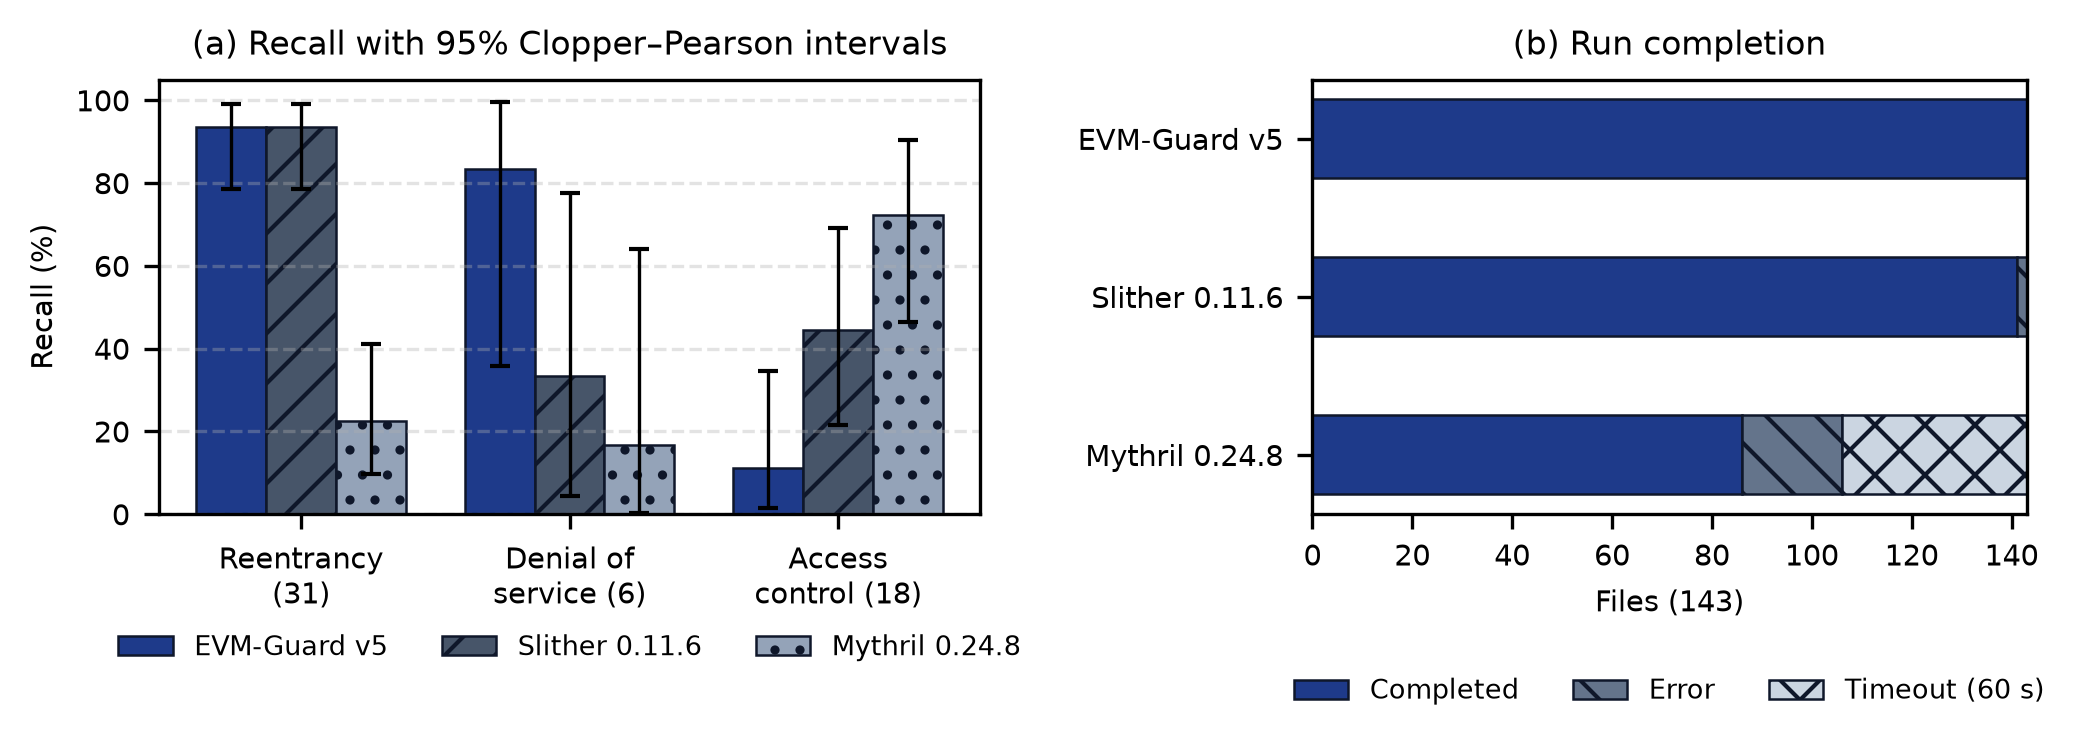
\includegraphics[width=\textwidth]{fig_smartbugs_empirical.png}
\caption{Results on SmartBugs-curated (143 files). (a) Recall of EVM-Guard v5, Slither 0.11.6 and Mythril 0.24.8 for reentrancy, denial of service and access control, with exact 95\% Clopper--Pearson intervals; arithmetic is reported in Table~\ref{tab:detection}. (b) Run completion: Mythril timed out on 37 files (25.9\%) and failed on 20, whereas EVM-Guard completed all 143.}
\label{fig:smartbugs_empirical}
\end{figure*}

Table~\ref{tab:detection} and Figure~\ref{fig:smartbugs_empirical} present the results for every scored category and all three tools. Differences between tools were tested with the paired McNemar test described in Section~\ref{sec:results:protocol}.

\paragraph{Reentrancy.} The figures in Table~\ref{tab:detection} refer to the final engine v5 and are post hoc. EVM-Guard v5 reached 93.5\% recall (29 of 31, CI [78.6, 99.2]) at 80.6\% precision, whereas engine v2, before the stipend correction, had the same recall at 53.7\% precision (Section~\ref{sec:results:correction}). Slither also reached 93.5\% recall, with the same 29 true positives, but its precision was 48.3\%; Mythril reached 22.6\% recall (7 of 31, CI [9.6, 41.1]). EVM-Guard v5 produced 7 false positives (FPR 6.2\%) and Slither 31 (FPR 27.7\%). Of the 112 negatives, 24 were flagged by Slither alone and none by v5 alone (McNemar $p = 1.2 \times 10^{-7}$); against Mythril, the corresponding counts were 4 and 27 ($p = 3.4 \times 10^{-5}$). This difference from Slither, however, disappears under the strict mapping (Section~\ref{sec:baselines}). Most of the 25 false positives of engine v2 arose from calls that forward only the stipend, which v3 and v5 exclude.

\paragraph{Reentrancy errors of v5.} Each of the remaining errors was examined individually. All seven false positives are files labelled as unchecked low-level calls, and Slither flags all seven as well. One of them is a genuine reentrancy that the label omits: \texttt{withdraw()} in \texttt{keepMyEther} sends the caller's balance with \texttt{call.value} and sets it to zero only afterwards. Three can be reached only by a privileged caller, since \texttt{sendTokenAw} in daoPOLSKA and \texttt{WithdrawToHolder} in TokenBank are restricted to the owner and \texttt{deliver} in TownCrier may be called only by its SGX address. In the remaining three, the callee is fixed by the owner: \texttt{donate} in two copies of PoCGame pays an address set by the owner, and CryptoPanda calls contracts configured by its CEO. Since engine v5 has no attacker model, it reports all six of these cases, whereas engine v6 removes the three privileged-caller cases and both copies of PoCGame (Section~\ref{sec:v6}). Of the two false negatives, \texttt{reentrancy\_bonus} is missed because its write lies in an internal function that is reached through a shared return address, which v5 merges, and \texttt{spank\_chain\_payment} is missed because its vulnerable contract contains an unlinked library placeholder and is not analysed (Section~\ref{sec:results:runtime}).

\paragraph{Denial of service.} EVM-Guard flagged 5 of the 6 labelled files (83.3\% recall, CI [35.9, 99.6]), Slither 2 (33.3\%, CI [4.3, 77.7]) and Mythril 1 (16.7\%, CI [0.4, 64.1]). With only six positives, these differences in recall cannot be regarded as established. EVM-Guard produced 34 false positives (12.8\% precision, FPR 24.8\%), against an FPR of 10.2\% for Slither and 17.5\% for Mythril. The loop check requires only an exit test derived from storage within a public function region, which may explain its false positives.

\paragraph{Access control.} Mythril achieved the highest recall in this category, 72.2\% (13 of 18, CI [46.5, 90.3]), at 54.2\% precision, followed by Slither with 44.4\% (8 of 18, CI [21.5, 69.2]) at 17.8\% precision. EVM-Guard flagged 2 of the 18 files (11.1\%, CI [1.4, 34.7]) and produced no false positive. Several access-control files rely on patterns that EVM-Guard does not target, such as authorisation through \texttt{tx.origin} (2 of the 18 labelled files) and unprotected self-destructs. Its delegatecall and proxy checks produced no false positive on this corpus, but they cover only direct call-hijacking hazards.

\paragraph{Arithmetic (construct mismatch).}\label{sec:results:arith} SmartBugs uses the arithmetic category for integer overflow and underflow, whereas the SWC-101 check of EVM-Guard targets division truncation. This row therefore shows how the truncation check behaves on code labelled for overflow; it does not measure the detection of truncation. EVM-Guard flagged 1 of the 15 labelled files (6.7\%, CI [0.2, 31.9]) and 80 other files, giving 1.2\% precision and a false-positive rate of 62.5\%. This high rate is consistent with the predicate of Definition~\ref{prop:prec}, which holds for almost any division that leaves a remainder. Neither Slither nor Mythril reported an overflow on this corpus (0\% recall, CI [0.0, 21.8]). Slither has no overflow detector, so the protocol maps none of its findings to arithmetic; Mythril completed 12 of the 15 arithmetic files (with 2 errors and 1 timeout), yet reported no SWC-101 finding on any of the 143 files.

\paragraph{Summary.} In summary, engine v5 reached 80.6\% reentrancy precision on this corpus (post hoc) and 100\% precision on access control, although the latter rests on only two flagged files. Precision was considerably lower for denial of service (12.8\%) and arithmetic (1.2\%), which is consistent with the conservative abstractions used for loops and truncation. Reentrancy is the only category in which the engine matched the recall of Slither. Outside reentrancy, v2, v3 and v5 flag the same files.

\subsection{Replay-Confirmed Findings}\label{sec:results:replay}
Across the 216 runtime contracts, engine v5 produced 194 static findings, 86 of which belong to the four classes that have a replay oracle (Table~\ref{tab:replay}). The oracles confirmed 8 of these findings: 4 for reentrancy, 3 for loop gas and 1 for delegatecall. All four confirmed reentrancy findings and the confirmed access-control finding are true positives with respect to the file labels, whereas the three confirmed denial-of-service findings include one false alarm (66.7\% precision). Overall, 7 of the 8 confirmed findings are true positives, a confirmation precision of 87.5\%. Recall on the confirmed findings alone is low: 12.9\% for reentrancy, 33.3\% for denial of service and 5.6\% for access control (Table~\ref{tab:replay_scores}). This is to be expected, since the oracles confirm only those hazards whose exploit can be reconstructed from the recovered selectors with generic attacker or probe contracts; a finding whose exploit requires specific arguments remains unconfirmed even when the static finding is correct. Replay therefore acts as a filter of high precision rather than as a means of finding hazards. With respect to the second research question, the oracle does not confirm warnings without false alarms, since one of the 8 confirmed findings is a false alarm, and recall falls to between 5.6\% and 33.3\% when only confirmed findings are counted.

\subsection{Case Studies from the Corpus}\label{sec:case_studies}
The two cases below are SmartBugs-curated contracts that EVM-Guard flags and the replay oracle confirms; line numbers refer to the sources in the dataset.

\paragraph{Reentrancy: \texttt{simple\_dao.sol} (labelled reentrancy).} \texttt{SimpleDAO} keeps a \texttt{credit} mapping. Its \texttt{withdraw(uint)} function checks the balance (line 17), calls \texttt{msg.sender.call.value(amount)()} (line 19) and only then decrements \texttt{credit[msg.sender]} (line 20), so the external call precedes the storage write. EVM-Guard recovers the dispatcher selectors, finds a CFG path from the \texttt{CALL} block to the \texttt{SSTORE} block within the region of \texttt{withdraw}, finds no mutex on that path, and reports SWC-107. During replay, the attacker first calls \texttt{donate(attacker)} with 1 ether, which credits its address, and then calls \texttt{withdraw} for 1 ether. The transfer from the victim re-enters the attacker, which calls \texttt{withdraw} again before the balance has been decremented. The attacker ends the transaction with 2 ether on a deposit of 1 ether, and the oracle therefore confirms the finding.

\paragraph{Loop gas: \texttt{dos\_address.sol} (labelled denial of service).} \texttt{DosGas} keeps a dynamic array, \texttt{creditorAddresses}, at storage slot 0. The public function \texttt{addCreditors} pushes 350 entries per call, and the public function \texttt{emptyCreditors} checks \texttt{creditorAddresses.length > 1500} and then clears the array. EVM-Guard reports a loop in the region of \texttt{emptyCreditors} (selector \texttt{0x0d870b7f}) whose exit test reads storage slot 0, the length of the array, and whose function is not guarded by a \texttt{CALLER} check. During replay, the oracle sets slot 0 to $10^6$, after which a call to \texttt{emptyCreditors} exhausts the limit of $G_{\mathrm{sandbox}} = 1.5\times10^6$ gas, whereas the same call on the original storage completes. This confirms unbounded growth at the reduced scale of the sandbox. The result is consistent with $\Phi_{\mathrm{DoS}}(G_{\mathrm{block}})$, but it does not show that a full block of 30 million gas would be exhausted.

\subsection{Evaluation on the SolidiFI Bug-Injection Benchmark}\label{sec:results:heldout}
In order to assess generalisation to an independent corpus, EVM-Guard was evaluated on the SolidiFI benchmark~\cite{ghaleb2020how}, which injects bugs of seven types into 50 base contracts (50 files per type) and also provides the 50 clean base contracts. The protocol (\texttt{docs/HELDOUT\_EVAL\_PROTOCOL.md}, with its SHA-256 digest in \texttt{docs/HELDOUT\_EVAL\_FREEZE.sha256}) fixed the corpus commits, the label mappings and the compiler settings before the analysis. Only reentrancy and arithmetic are scored, since EVM-Guard has no detector for the other injected types and the corpus contains no denial-of-service or delegatecall class. All 400 files compiled with solc 0.5.12, yielding 984 runtime contracts, and the baselines were run with the same settings as on SmartBugs.

The held-out run used engine v2, which flagged all 50 reentrancy files (100\%, CI [92.9, 100]) together with 130 false positives, a precision of 27.8\% and a false-positive rate of 37.1\%. Table~\ref{tab:heldout} reports the final engine v5, whose figures are post hoc: it produced 35 false positives, giving 58.8\% precision and a false-positive rate of 10.0\%, the same as v3. Slither flagged all 50 positives with 150 false positives (25.0\% precision, FPR 42.9\%). Mythril finished only 84 of the 400 files (308 timeouts and 8 errors) and flagged 2 of the 50 reentrancy files (4\% recall, 22.2\% precision, FPR 2.0\%). Since every SolidiFI file is derived from one of the same 50 base contracts, some false positives probably reflect reentrancy patterns that are already present in the unlabelled base code. On the 50 clean contracts alone, v2 flagged 6 for reentrancy (12\%) and v5 flagged 5 (10\%).

The arithmetic row again reflects the mismatch between overflow labels and a truncation check. EVM-Guard flagged 45 of the 50 files with injected overflows (90\%), but it also flagged 45 of the 50 clean contracts, because of division truncation in the shared base code. Of the 350 files without an arithmetic label, 315 were flagged (FPR 90.0\%, precision 12.5\%). Neither Slither nor Mythril reported an arithmetic finding.

Replay confirmed no reentrancy finding on this corpus, although it confirmed 16 SWC-128 findings, which are not scored here. In the file that was examined (\texttt{Re-entrancy/buggy\_1.sol}), the injected withdrawal functions pay out from per-sender balance mappings that no function of the contract credits; in a fresh sandbox, the attacker therefore has no balance to withdraw, and the gain criterion cannot be met. The same contract also exposes 29 selectors, more than the limit of 8 candidates used by the oracle. The absence of confirmations on this corpus therefore reflects the limited reach of the oracle rather than an absence of the injected bugs.

Since the engine was changed after this run (v3 and v5), the SolidiFI figures for those versions are post hoc, and a fair test of an improvement in precision requires a corpus that has not yet been used.

\subsection{Evaluation on a Labelled Benchmark Suite}\label{sec:results:heldout2}
SolidiFI has no denial-of-service, tx.origin or SELFDESTRUCT class, and its files share 50 base contracts. EVM-Guard was therefore also evaluated on an open repository of labelled contracts\footnote{\url{https://github.com/bit-smartcontract-analysis/smartcontract-benchmark}} at commit \texttt{8b903aa}, whose 389 Solidity files are labelled by folder: reentrancy (81), arithmetic (65), unsafe delegatecall (12), tx.origin (10), unsafe SELFDESTRUCT (11), and five further classes (unchecked send, TOD, time manipulation, bad randomness, gasless send), plus 17 safe contracts. The evaluation protocol (\texttt{docs/HELDOUT2\_EVAL\_PROTOCOL.md}, with its SHA-256 digest in \texttt{docs/HELDOUT2\_EVAL\_FREEZE.sha256}) fixed the mappings between labels and categories and the compiler configurations, and the catalogue records the commit and the SHA-256 digest of each source.

The folder labels were mapped to the SmartBugs categories as follows. Reentrancy corresponds to SWC-107 and arithmetic to SWC-101, with the same mismatch between overflow and truncation as before. Access control groups the delegatecall folder (SWC-112), the tx.origin folder (SWC-115) and the SELFDESTRUCT folder (SWC-106), as in the SmartBugs mapping; since EVM-Guard has no check for tx.origin or SELFDESTRUCT, those 21 files can only count as misses. The five remaining classes are negatives for every scored category. Denial of service is not evaluated, because no file carries that label. Thirteen files do not compile with the available compilers; they remain in the scoring as unflagged.

\begin{table}[t]
\centering
\small
\caption{Results on the labelled benchmark (389 files, of which 376 compile; the other 13 count as unflagged). EVM-Guard rows refer to the final engine v5 and are post hoc; the results of the held-out engine v2 are given in the text. Recall, precision and FPR with exact 95\% Clopper--Pearson intervals. Denial of service is not evaluated, because the benchmark has no such label.}
\label{tab:heldout2}
\resizebox{\columnwidth}{!}{%
\begin{tabular}{@{}llrrrrr@{}}
\toprule
\textbf{Category} & \textbf{Tool} & \textbf{TP} & \textbf{FP} & \textbf{Recall [CI]} & \textbf{Precision [CI]} & \textbf{FPR [CI]} \\
\midrule
Reentrancy (81 pos.) & \textbf{EVM-Guard} & 79 & 25 & 97.5 [91.4, 99.7] & 76.0 [66.6, 83.8] & 8.1 [5.3, 11.7] \\
 & Slither & 79 & 111 & 97.5 [91.4, 99.7] & 41.6 [34.5, 48.9] & 36.0 [30.7, 41.7] \\
 & Mythril & 14 & 32 & 17.3 [9.8, 27.3] & 30.4 [17.7, 45.8] & 10.4 [7.2, 14.3] \\
\midrule
Arithmetic (65 pos.) & \textbf{EVM-Guard} & 46 & 245 & 70.8 [58.2, 81.4] & 15.8 [11.8, 20.5] & 75.6 [70.6, 80.2] \\
 & Slither & 0 & 0 & 0.0 [0.0, 5.5] & n/a & 0.0 [0.0, 1.1] \\
 & Mythril & 0 & 0 & 0.0 [0.0, 5.5] & n/a & 0.0 [0.0, 1.1] \\
\midrule
Access control (33 pos.) & \textbf{EVM-Guard} & 7 & 0 & 21.2 [9.0, 38.9] & 100.0 [59.0, 100.0] & 0.0 [0.0, 1.0] \\
 & Slither & 22 & 152 & 66.7 [48.2, 82.0] & 12.6 [8.1, 18.5] & 42.7 [37.5, 48.0] \\
 & Mythril & 11 & 25 & 33.3 [18.0, 51.8] & 30.6 [16.3, 48.1] & 7.0 [4.6, 10.2] \\
\bottomrule
\end{tabular}%
}
\end{table}


The held-out run again used engine v2, which reached 97.5\% reentrancy recall (79 of 81) at 46.2\% precision (CI [38.6, 54.0]) and a false-positive rate of 29.9\%. The final engine v5 (Table~\ref{tab:heldout2}, post hoc) has the same recall at 76.0\% precision (CI [66.6, 83.8]) and a false-positive rate of 8.1\%. Slither matched this recall at 41.6\% precision and a false-positive rate of 36.0\%. Mythril completed 143 of the 389 files (231 timeouts and 15 errors) and reached 17.3\% recall; a rerun with a limit of 300\,s completed only 2 of the 231 files that had timed out, which raised its access-control recall from 33.3\% to 39.4\% and left reentrancy unchanged. Of the 92 reentrancy false positives of v2, 58 lie in the TOD folder, compared with 5 of the 25 of v5. These files were scored as negatives on the basis of their label, without manual review.

For access control, EVM-Guard v5 flagged 7 files, all in the delegatecall folder, without a false positive (v2 had flagged 6). Its recall over the 33 positives is 21.2\%, since the tx.origin and SELFDESTRUCT files lie outside its checks; Slither reached 66.7\% recall at 12.6\% precision, and Mythril 33.3\% recall at 30.6\% precision. In the arithmetic category, where overflow labels are again compared with a truncation check, EVM-Guard v5 flagged 46 of the 65 overflow files (70.8\% recall) and 245 of the 324 negatives (FPR 75.6\%, precision 15.8\%), whereas neither Slither nor Mythril reported an arithmetic finding. Replay confirmed 4 reentrancy findings and 2 access-control findings, all of which are true positives.

On SolidiFI and on this benchmark, the reentrancy precision of v5 is thus 58.8\% and 76.0\%; both figures are post hoc.

\subsection{Ablation: Effect of the Gas-Stipend Bound}\label{sec:results:correction}
Solidity compiles \texttt{address.transfer} and \texttt{address.send} into a \texttt{CALL} whose gas operand is computed as $2300 \cdot \mathrm{ISZERO}(v)$ rather than given as a constant. Such calls forward at most the stipend of 2300 gas, which is not enough for the callee to modify storage. Before the Istanbul fork, \texttt{SSTORE} required at least 5,000 gas, and since EIP-2200 and EIP-2929 an explicit check halts execution with an out-of-gas error whenever the remaining gas is at most 2300. A call that forwards only the stipend therefore cannot re-enter the caller and modify its storage.

The effect of this exclusion was assessed by comparing EVM-Guard with and without the stipend bound. In the full engine, abstract stack values carry sound upper bounds, which are propagated through \texttt{ISZERO} (bound 1), \texttt{MUL} (product of the bounds) and \texttt{AND} (the smaller bound), and any call whose bound does not exceed 2300 gas is excluded.

Table~\ref{tab:correction} compares reentrancy detection on the three real benchmarks for engine v2, the stipend-corrected engine v3 and the final engine v5. The stipend bound raised precision from 53.7\% to 78.4\% on SmartBugs-curated, from 27.8\% to 58.8\% on SolidiFI and from 46.2\% to 75.2\% on the labelled benchmark, while recall remained unchanged. The slot-based mutex rule of v5 removed one further false positive on SmartBugs-curated (80.6\%) and one on the labelled benchmark (76.0\%). All of these figures are post hoc. Of the 58 files in the TOD folder of the labelled benchmark that v2 flags for reentrancy, the stipend bound removes 53, and in each of these 53 sources value is sent only through \texttt{transfer} or \texttt{send}.

\begin{table}[t]
\centering
\small
\caption{Reentrancy (SWC-107) precision and FPR (\%) for engine v2 (no stipend bound), v3 (stipend bound) and v5 (final engine) on the three real benchmarks. All figures are post hoc. Recall is the same for the three versions on each benchmark.}
\label{tab:correction}
\resizebox{\columnwidth}{!}{%
\begin{tabular}{@{}lrrrrrr@{}}
\toprule
\textbf{Corpus (positives)} & \multicolumn{2}{c}{\textbf{v2}} & \multicolumn{2}{c}{\textbf{v3}} & \multicolumn{2}{c}{\textbf{v5}} \\
 & Prec. & FPR & Prec. & FPR & Prec. & FPR \\
\midrule
SmartBugs-curated (31) & 53.7 & 22.3 & 78.4 & 7.1 & \textbf{80.6} & \textbf{6.2} \\
SolidiFI (50) & 27.8 & 37.1 & 58.8 & 10.0 & \textbf{58.8} & \textbf{10.0} \\
Labelled benchmark (81) & 46.2 & 29.9 & 75.2 & 8.4 & \textbf{76.0} & \textbf{8.1} \\
\bottomrule
\end{tabular}%
}
\end{table}

In addition, the components of the final engine were disabled one at a time on SmartBugs-curated (\texttt{results/ablation/}). This ablation covers reentrancy only, and recall was unchanged in every configuration. Removing the stipend exclusion, or applying it only to constant gas operands, raised the number of false positives from 7 to 22 (56.9\% precision). Removing the slot-based mutex rule raised it to 8 (78.4\%), and removing both mutex rules gave the same result. Disabling the \texttt{PUSH0} decoder, the removal of the CBOR trailer, or the dominance requirement of the mutex rule did not change any reentrancy flag. A configuration that reproduces engine v2 gave 25 false positives (53.7\%), in agreement with the archived v2 run for every file.

\subsection{First Pre-Registered Synthetic Test (Engine v3)}\label{sec:results:fresh}
This test applied engine v3 to a corpus that had not been used at any stage of development. The protocol (\texttt{docs/INJECTED05\_EVAL\_PROTOCOL.md}), together with its generator, catalogue and engine manifest, was frozen before the run, and the digests are recorded in \texttt{docs/INJECTED05\_EVAL\_FREEZE.sha256}. The corpus consists of 210 contracts compiled with solc 0.5.12, in seven groups of 30: positives with an injected reentrancy or denial-of-service pattern, and five groups of negatives (checks before effects, a mutex-guarded call, a payout through \texttt{transfer}, a bounded loop, and no injected pattern). Since the labels are assigned by construction and the families are few, the test measures the detector on its own injection patterns and provides no evidence about real contracts; its purpose was to measure precision on a fresh sample.

The results are shown in Table~\ref{tab:fresh}. For reentrancy, EVM-Guard flagged all 30 injected contracts, and all of its 30 false positives belong to the mutex-guarded group; the checks-before-effects, \texttt{transfer} and bounded-loop groups produced none. Slither and Mythril also flagged all 30 positives, with 60 and 57 false positives respectively. For denial of service, EVM-Guard flagged all 30 injected contracts without a false positive, whereas Slither and Mythril flagged none of them. Mythril timed out on 3 of the 210 files, which count as unflagged.

\begin{table}[t]
\centering
\small
\caption{First pre-registered synthetic test (210 Solidity 0.5.12 contracts, engine v3). Recall, precision and FPR with exact 95\% Clopper--Pearson intervals. Each category is scored on its own positives and negatives.}
\label{tab:fresh}
\resizebox{\columnwidth}{!}{%
\begin{tabular}{@{}llrrrrr@{}}
\toprule
\textbf{Category (positives)} & \textbf{Tool} & \textbf{TP} & \textbf{FP} & \textbf{Recall [CI]} & \textbf{Precision [CI]} & \textbf{FPR [CI]} \\
\midrule
Reentrancy (30) & EVM-Guard & 30 & 30 & 100.0 [88.4, 100.0] & 50.0 [36.8, 63.2] & 16.7 [11.5, 22.9] \\
 & Slither & 30 & 60 & 100.0 [88.4, 100.0] & 33.3 [23.7, 44.1] & 33.3 [26.5, 40.7] \\
 & Mythril & 30 & 57 & 100.0 [88.4, 100.0] & 34.5 [24.6, 45.4] & 31.7 [24.9, 39.0] \\
\midrule
Denial of service (30) & EVM-Guard & 30 & 0 & 100.0 [88.4, 100.0] & 100.0 [88.4, 100.0] & 0.0 [0.0, 2.0] \\
 & Slither & 0 & 0 & 0.0 [0.0, 11.6] & n/a & 0.0 [0.0, 2.0] \\
 & Mythril & 0 & 0 & 0.0 [0.0, 11.6] & n/a & 0.0 [0.0, 2.0] \\
\bottomrule
\end{tabular}%
}
\end{table}

The cause of the mutex failure could be identified. In the mutex-guarded contracts, \texttt{locked} is written through a masked read-modify-write, so the stored value is not the constant that the mutex rule expects and the guard is not recognised. The engine was not changed on the basis of this corpus, since the corpus would then have been spent; the corrected mutex rule was instead tested on a new pre-registered corpus (Section~\ref{sec:results:final}).


\subsection{Final Pre-Registered Synthetic Test (Engine v5)}\label{sec:results:final}
The final engine, v5, consists of v3 with the \texttt{PUSH0} decoder and the slot-based mutex rule. It contains no return-site fallback, because that fallback lowered precision on the real benchmarks (SmartBugs reentrancy from 78.4\% to 55.6\%, SolidiFI from 58.8\% to 23.6\%). Under Protocol~6 (\texttt{docs/FINAL\_V5\_EVAL\_PROTOCOL.md}, frozen before the run, with digests in \texttt{docs/FINAL\_V5\_EVAL\_FREEZE.sha256}), this engine was run once on a new corpus of 210 contracts compiled with solc 0.5.12. Before that, Protocol~5 (\texttt{docs/FRESH\_V4\_EVAL\_PROTOCOL.md}) had tested an intermediate engine, v4, which included the return-site fallback, on two further corpora of 210 contracts, \texttt{injected05b} (solc 0.5.12) and \texttt{injected8b} (solc 0.8.20). Table~\ref{tab:protocol5} reports that run as it was frozen. Engine v4 was not adopted, because its fallback lowered precision on the real benchmarks, and both of its corpora are now spent. The corpus of Protocol~6 has the same seven groups as before and had not been used for any engine version. As its labels are assigned by construction, the result again concerns the injection patterns of the detector and not precision on real contracts. Table~\ref{tab:final} reports the results.

\begin{table}[t]
\centering
\small
\caption{Final pre-registered synthetic test (Protocol~6; 210 Solidity 0.5.12 contracts). Recall, precision and FPR with exact 95\% Clopper--Pearson intervals. Mythril had 12 timeouts and 1 error, which count as unflagged.}
\label{tab:final}
\resizebox{\columnwidth}{!}{%
\begin{tabular}{@{}llrrrrr@{}}
\toprule
\textbf{Category (positives)} & \textbf{Tool} & \textbf{TP} & \textbf{FP} & \textbf{Recall [CI]} & \textbf{Precision [CI]} & \textbf{FPR [CI]} \\
\midrule
Reentrancy (30) & EVM-Guard v5 & 30 & 0 & 100.0 [88.4, 100.0] & 100.0 [88.4, 100.0] & 0.0 [0.0, 2.0] \\
 & Slither & 30 & 60 & 100.0 [88.4, 100.0] & 33.3 [23.7, 44.1] & 33.3 [26.5, 40.7] \\
 & Mythril & 30 & 47 & 100.0 [88.4, 100.0] & 39.0 [28.0, 50.8] & 26.1 [19.9, 33.2] \\
\midrule
Denial of service (30) & EVM-Guard v5 & 30 & 0 & 100.0 [88.4, 100.0] & 100.0 [88.4, 100.0] & 0.0 [0.0, 2.0] \\
 & Slither & 0 & 0 & 0.0 [0.0, 11.6] & n/a & 0.0 [0.0, 2.0] \\
 & Mythril & 0 & 0 & 0.0 [0.0, 11.6] & n/a & 0.0 [0.0, 2.0] \\
\bottomrule
\end{tabular}%
}
\end{table}

\begin{table}[t]
\centering
\small
\caption{Protocol~5: intermediate engine v4 (return-site fallback) on two pre-registered synthetic corpora of 210 contracts (30 reentrancy, 30 denial of service, 150 negatives). Precision with exact 95\% Clopper--Pearson intervals; recall is 100\% wherever TP is 30. Engine v4 was not adopted.}
\label{tab:protocol5}
\resizebox{\columnwidth}{!}{%
\begin{tabular}{@{}llrrlrrl@{}}
\toprule
 & & \multicolumn{3}{c}{\textbf{Reentrancy}} & \multicolumn{3}{c}{\textbf{Denial of service}} \\
\textbf{Corpus} & \textbf{Tool} & TP & FP & Precision [CI] & TP & FP & Precision [CI] \\
\midrule
\texttt{injected05b} & EVM-Guard v4 & 30 & 0 & 100.0 [88.4, 100.0] & 30 & 0 & 100.0 [88.4, 100.0] \\
(solc 0.5.12) & Slither & 30 & 60 & 33.3 [23.7, 44.1] & 0 & 0 & n/a \\
 & Mythril & 30 & 54 & 35.7 [25.6, 46.9] & 0 & 0 & n/a \\
\midrule
\texttt{injected8b} & EVM-Guard v4 & 30 & 60 & 33.3 [23.7, 44.1] & 0 & 0 & n/a \\
(solc 0.8.20) & Slither & 30 & 60 & 33.3 [23.7, 44.1] & 0 & 0 & n/a \\
 & Mythril & 30 & 60 & 33.3 [23.7, 44.1] & 0 & 0 & n/a \\
\bottomrule
\end{tabular}%
}
\end{table}

On Solidity 0.5.12, engine v4 obtained the same result as v5 later did. On Solidity 0.8.20, its fallback, which links every return of a shared helper to every caller, allowed it to reach the call sites, but it also flagged all 60 mutex-guarded and checks-before-effects negatives and found none of the denial-of-service contracts. Engine v6 replaces this fallback with return sites tracked per context (Section~\ref{sec:arch:v6}).

The denial-of-service result shows that the baselines do not flag this template; it does not show that EVM-Guard detects denial of service in real contracts. On the earlier synthetic corpus (Section~\ref{sec:results:fresh}), where v3 had reached 50\% precision because of the mutex defect, v5 also scores 100\%, but that figure is post hoc, since the corpus had already been used.

\subsection{Runtime and Completion}\label{sec:results:runtime}
Table~\ref{tab:runtime} reports the run outcomes and the wall time per file for the analysis stage, excluding replay. EVM-Guard completed all 143 files without a timeout or an error, with a median analysis time of 87\,ms (mean 128\,$\pm$\,170\,ms). Slither completed 141 files and failed on 2, with a median of 289\,ms (mean 304\,$\pm$\,135\,ms), and Mythril completed 86 files, with 37 timeouts (25.9\%) and 20 crashes and a median of 26,025\,ms (mean 30,288\,$\pm$\,24,942\,ms). It should be noted that the times of the baselines include compilation from source, whereas EVM-Guard analyses compiled bytecode. One of the 216 runtime contracts, \texttt{LedgerChannel} in \texttt{spank\_chain\_payment.sol}, contains an unlinked library placeholder and is not analysed, so its file is scored on its other contracts. When the placeholder is linked, the file is also flagged for reentrancy, and reentrancy recall rises to 96.8\% (30 of 31, CI [83.3, 99.9]) at 81.1\% precision. Since unfinished files count as unflagged, the timeouts and errors of Mythril lower its recall in Table~\ref{tab:detection}.

%% ===========================================================================
\section{Comparison with Bytecode Analysers and a Strict Slither Mapping}\label{sec:baselines}

\paragraph{Setup.} All of the tools discussed in this section were run on the same files as EVM-Guard, and the run files are available in \texttt{results/baselines\_round3/}. Slither 0.11.6 was run again with its detector names recorded, so that the same run could be scored under the mapping of Addendum~A and under the strict mapping (Section~\ref{sec:results:protocol}). EVMLiSA (commit \texttt{44ae6dd}, built with JDK~21) received the same runtime bytecode as EVM-Guard, with the solc metadata trailer removed, since EVMLiSA otherwise stops on the truncated \texttt{PUSH} instruction to which the trailer decodes; it was given 60\,s per runtime contract (\texttt{src/eval/run\_evmlisa.py}). As the download links of the eThor authors were no longer available, the SmartBugs image \texttt{smartbugs/ethor:2023} was used with the SmartBugs command line. This image is built for amd64 only and therefore ran under emulation on the arm64 evaluation machine, which is why it was given 120\,s per contract. At a mean of 25\,s per file under emulation, and with no more than three containers in memory at a time, eThor was run on SmartBugs-curated and on the Protocol~6 synthetic corpus; within the time available, it was not run on SolidiFI and the labelled benchmark (a further 1,764 runtime contracts). Sailfish analyses source code, and its symbolic verifier is a Racket program. In the authors' image (\texttt{holmessherlock/sailfish}), the Racket runtime aborted on the evaluation machine under both QEMU and Rosetta emulation, even for the command \texttt{racket -e "(display 1)"}, so the complete tool could not be run. Its static stage, which proposes the candidates that the verifier would refine, was run instead. Since the verifier can only remove candidates, the recall of the static stage is an upper bound on the recall of the complete tool. In all cases, a file is flagged if the tool reports at least one reentrancy finding on any of its contracts.

\begin{table*}[t]
\centering
\small
\caption{Reentrancy against Slither under two mappings and three further analysers, on the same files. Mapped Slither counts every \texttt{reentrancy-*} detector; strict Slither counts \texttt{reentrancy-eth} and \texttt{reentrancy-no-eth}. EVMLiSA had 60\,s and eThor 120\,s per runtime contract; files a tool did not finish count as unflagged, and the last column gives how many. The McNemar column compares false positives with EVM-Guard v5 (and v6 where it was run): files flagged only by EVM-Guard / only by the tool, with the two-sided $p$-value. Sailfish's static stage is reported only on SmartBugs-curated, because it crashed on most reentrancy-positive files of the other corpora (text). eThor was run on two corpora only (text).}
\label{tab:baselines}
\resizebox{\textwidth}{!}{%
\begin{tabular}{@{}llrrrllr@{}}
\toprule
\textbf{Corpus (pos./files)} & \textbf{Tool} & TP & FP & Recall & Precision [CI] & FP vs v5 / vs v6 ($p$) & Unfinished \\
\midrule
SmartBugs-curated (31/143) & EVM-Guard v5 & 29 & 7 & 93.5 & 80.6 [64.0, 91.8] & -- & 0 \\
 & Slither, mapped & 29 & 31 & 93.5 & 48.3 [35.2, 61.6] & 0/24 ($1.2 \times 10^{-7}$) & 2 \\
 & Slither, strict & 29 & 9 & 93.5 & 76.3 [59.8, 88.6] & 2/4 (0.69) & 2 \\
 & EVMLiSA & 30 & 25 & 96.8 & 54.5 [40.6, 68.0] & 1/19 ($4 \times 10^{-5}$) & 4 \\
 & eThor & 30 & 60 & 96.8 & 33.3 [23.7, 44.1] & 5/58 ($1.7 \times 10^{-12}$) & 27 \\
 & Sailfish, static stage & 24 & 4 & 77.4 & 85.7 [67.3, 96.0] & 4/1 (0.38) & 5 \\
\midrule
SolidiFI (50/400) & EVM-Guard v5 & 50 & 35 & 100.0 & 58.8 [47.6, 69.4] & -- & 0 \\
 & EVM-Guard v6 & 50 & 56 & 100.0 & 47.2 [37.4, 57.1] & -- & 0 \\
 & Slither, mapped & 50 & 150 & 100.0 & 25.0 [19.2, 31.6] & 0/115 ($4.8 \times 10^{-35}$) / 0/94 ($1 \times 10^{-28}$) & 0 \\
 & Slither, strict & 50 & 42 & 100.0 & 54.4 [43.6, 64.8] & 0/7 (0.016) / 14/0 ($1.2 \times 10^{-4}$) & 0 \\
 & EVMLiSA & 37 & 71 & 74.0 & 34.3 [25.4, 44.0] & 20/56 ($4.4 \times 10^{-5}$) / 34/49 (0.12) & 111 \\
\midrule
Labelled (81/389) & EVM-Guard v5 & 79 & 25 & 97.5 & 76.0 [66.6, 83.8] & -- & 0 \\
 & EVM-Guard v6 & 79 & 35 & 97.5 & 69.3 [60.0, 77.6] & -- & 0 \\
 & Slither, mapped & 79 & 111 & 97.5 & 41.6 [34.5, 48.9] & 1/87 ($5.8 \times 10^{-25}$) / 0/76 ($2.6 \times 10^{-23}$) & 14 \\
 & Slither, strict & 79 & 29 & 97.5 & 73.2 [63.8, 81.2] & 5/9 (0.42) / 10/4 (0.18) & 14 \\
 & EVMLiSA & 68 & 53 & 84.0 & 56.2 [46.9, 65.2] & 12/40 ($1.3 \times 10^{-4}$) / 20/38 (0.025) & 90 \\
\midrule
Synthetic, Protocol 6 (30/210) & EVM-Guard v5 & 30 & 0 & 100.0 & 100.0 [88.4, 100.0] & -- & 0 \\
 & Slither, mapped & 30 & 60 & 100.0 & 33.3 [23.7, 44.1] & 0/60 ($1.7 \times 10^{-18}$) & 0 \\
 & Slither, strict & 30 & 30 & 100.0 & 50.0 [36.8, 63.2] & 0/30 ($1.9 \times 10^{-9}$) & 0 \\
 & EVMLiSA & 30 & 60 & 100.0 & 33.3 [23.7, 44.1] & 0/60 ($1.7 \times 10^{-18}$) & 0 \\
 & eThor & 30 & 87 & 100.0 & 25.6 [18.0, 34.5] & 0/87 ($1.3 \times 10^{-26}$) & 7 \\
\bottomrule
\end{tabular}%
}
\end{table*}


\paragraph{Results.} The comparison is presented in Table~\ref{tab:baselines}. Under the strict mapping, the false positives of Slither fall from 31 to 9 on SmartBugs-curated, from 150 to 42 on SolidiFI and from 111 to 29 on the labelled benchmark, without any loss of recall. Against strict Slither, v5 has significantly fewer false positives only on SolidiFI (7 negatives flagged by strict Slither alone and none by v5 alone, $p = 0.016$) and on the synthetic corpus. On SmartBugs-curated (2 negatives flagged by v5 alone and 4 by Slither alone, $p = 0.69$) and on the labelled benchmark (5 and 9, $p = 0.42$), the difference is not significant, and on SolidiFI v6 has significantly more false positives than strict Slither (14 and none, $p = 1.2 \times 10^{-4}$). The comparisons with mapped Slither in Section~\ref{sec:results:detection} therefore depend on the mapping, and the comparison with strict Slither is the more appropriate one. EVMLiSA and eThor flag almost every positive, but both produce significantly more false positives than v5 on every corpus on which they were run. eThor attempts to prove single-entrancy, a stronger property than exploitable reentrancy, and reports a contract as insecure whenever the proof fails, which is likely to account for its false positives; it also failed to finish 27 SmartBugs files (21 timeouts and 6 crashes). EVMLiSA timed out on 111 SolidiFI files and 76 labelled files at 60\,s, and 13 labelled files have no bytecode because their sources do not compile, which lowers its recall on those corpora. With a limit of 600\,s, and with a build that omits the CFG dump (which crashes on some graphs after the analysis has finished, and whose omission left the findings unchanged on 20 files that the standard build completes), EVMLiSA finished all SmartBugs-curated files, with 30 true and 28 false positives, and 55 of the 58 SolidiFI files that were rerun. Its false positives remained significantly more numerous than those of v5 ($p = 9.5 \times 10^{-7}$ and $2.2 \times 10^{-12}$). The static stage of Sailfish completed 138 SmartBugs files with 24 true and 4 false positives (85.7\% precision, 77.4\% recall). Its false positives do not differ significantly from those of v5 (4 negatives flagged by v5 alone and 1 by Sailfish alone, $p = 0.38$); it misses 7 positives that v5 finds and finds 2 that v5 misses. On the other corpora, however, it stopped with an internal assertion (``ORed count does not match'') in its value-range analysis on all 50 SolidiFI reentrancy files, on 51 of the 81 labelled reentrancy files, and on all 30 injected-reentrancy and 30 mutex-guarded synthetic contracts. Scores on those corpora would therefore measure the failure rather than detection, and they are not reported.

%% ===========================================================================
\section{Engine v6 under a Pre-Registered Protocol}\label{sec:v6}

\paragraph{Protocol.} Engine v6 was developed on SmartBugs-curated, on five fixtures in \texttt{tests/fixtures/} and on the spent corpus \texttt{injected8b}, so its figures on these sets are post hoc. Protocol~7 (\texttt{docs/ENGINE\_V6\_EVAL\_PROTOCOL.md}) was then frozen; SHA-256 digests of the protocol, the labelling rubric, the corpus builders and the engine manifest are recorded in \texttt{docs/ENGINE\_V6\_EVAL\_FREEZE.sha256}, and byte copies of the v6 sources are kept in \texttt{archive/engine\_v6/}. The protocol specifies five corpora on which v6 had never been run: SolidiFI, the labelled benchmark, two new synthetic corpora built by the earlier generators with new seeds (\texttt{injected05d}, solc 0.5.12, seed 20261101; \texttt{injected8c}, solc 0.8.20, seed 20261102; 210 files each), and the deployed contracts described in Section~\ref{sec:v6:mainnet}. Each corpus was analysed once with the frozen v5 and v6 engines, and the protocol requires the results to be reported whatever they are. Two files outside the engine were changed after the freeze, in both cases before any engine had been run on the corpus concerned; the changes are recorded in \texttt{docs/ENGINE\_V6\_EVAL\_ADDENDUM.md}. The engine sources matched the manifest when the runs began.

\begin{table*}[t]
\centering
\small
\caption{Protocol~7: frozen engines v5 and v6 on the same files, reentrancy. Precision with exact 95\% Clopper--Pearson intervals (recall and FPR intervals are in \texttt{results/protocol7/scores.json}). The last two columns give the exact McNemar test of v5 against v6 on the negatives (FP) and on the positives (TP): files flagged by v5 only / by v6 only, and the two-sided $p$-value. Neither engine had been run on these corpora before the freeze, except v5 on SolidiFI and the labelled benchmark, whose v5 figures are post hoc.}
\label{tab:v6}
\resizebox{\textwidth}{!}{%
\begin{tabular}{@{}llrrrrlrll@{}}
\toprule
\textbf{Corpus (positives)} & \textbf{Engine} & TP & FP & FN & Recall & Precision [CI] & FPR & FP: v5/v6 only ($p$) & TP: v5/v6 only ($p$) \\
\midrule
SolidiFI (50) & v5 & 50 & 35 & 0 & 100.0 & 58.8 [47.6, 69.4] & 10.0 & 0/21 ($9.5 \times 10^{-7}$) & 0/0 (1) \\
 & v6 & 50 & 56 & 0 & 100.0 & 47.2 [37.4, 57.1] & 16.0 &  &  \\
\midrule
Labelled (81) & v5 & 79 & 25 & 2 & 97.5 & 76.0 [66.6, 83.8] & 8.1 & 3/13 (0.0213) & 1/1 (1) \\
 & v6 & 79 & 35 & 2 & 97.5 & 69.3 [60.0, 77.6] & 11.4 &  &  \\
\midrule
\texttt{injected05d}, 0.5.12 (30) & v5 & 30 & 0 & 0 & 100.0 & 100.0 [88.4, 100.0] & 0.0 & 0/0 (1) & 0/0 (1) \\
 & v6 & 30 & 0 & 0 & 100.0 & 100.0 [88.4, 100.0] & 0.0 &  &  \\
\midrule
\texttt{injected8c}, 0.8.20 (30) & v5 & 0 & 0 & 30 & 0.0 & n/a & 0.0 & 0/0 (1) & 0/30 ($1.9 \times 10^{-9}$) \\
 & v6 & 30 & 0 & 0 & 100.0 & 100.0 [88.4, 100.0] & 0.0 &  &  \\
\bottomrule
\end{tabular}%
}
\end{table*}


\paragraph{Results.} The reentrancy results are shown in Table~\ref{tab:v6}. On the two synthetic corpora, both engines are exact on Solidity 0.5.12, and on Solidity 0.8.20 v6 finds all 30 injected reentrancies without a false positive, whereas v5 finds none ($p = 1.9 \times 10^{-9}$). It is return-site tracking that makes 0.8 bytecode analysable. On the two real benchmarks, v6 retains the recall of v5 but adds false positives: 21 on SolidiFI ($p = 9.5 \times 10^{-7}$) and a net 10 on the labelled benchmark (13 added and 3 removed, $p = 0.021$). All 21 additional SolidiFI findings are classified as \emph{same-function, feasible}, and 7 of these files also carry an \emph{unknown} finding. The additional candidates therefore come from code that return-site tracking makes reachable, rather than from candidates that the solver failed to decide. Z3 confirms that a path to the call and a re-entrant run exist, but the attacker model cannot establish that re-entry would benefit the attacker; the callee may be, for example, a seller who would only pay itself. On the labelled benchmark, v6 also adds 6 arithmetic false positives ($p = 0.031$), which arise from the same newly reachable code. On \texttt{injected8c}, it flags all 30 denial-of-service positives together with all 30 bounded-loop negatives, which shows that its loop check does not carry over to 0.8 bytecode; no claim is made for denial of service.

\paragraph{Consequence.} Engine v6 is thus the better choice for Solidity 0.8 bytecode, and it records the kind of each reentrancy, but on Solidity 0.4--0.5 code it is significantly less precise than v5. For this reason, v5 is retained as the default engine, and the v5 figures elsewhere in this paper are unchanged. On SmartBugs-curated (post hoc), v6 reaches 29 true positives with 4 false positives (87.9\%). Compared with v5, it removes the three privileged-caller false positives and both copies of PoCGame discussed in Section~\ref{sec:results:detection}, finds \texttt{reentrancy\_bonus}, misses TokenBank, whose withdrawal function is restricted to the owner through a shadowed owner variable, and adds two unknown findings on Parity wallet files.

%% ===========================================================================
\section{Deployed Contracts}\label{sec:v6:mainnet}

\paragraph{Corpus.} The corpus was defined in the protocol before any engine was run on it. It consists of every entry of the smart-contract-sanctuary mainnet index (commit \texttt{015d0105}, index SHA-256 \texttt{fdb990d8\ldots}) compiled with Solidity 0.4 or 0.5, excluding the 37,892 addresses that appear anywhere in the earlier corpora, that held a non-zero ether balance and had code at a single block (\texttt{src/eval/build\_mainnet\_catalog.py}). Of the 43,998 candidates, 3,214 contracts held ether at block 26,319,084, 45,217 ether in total (median 0.011 ether; 413 contracts held at least 1 ether). The engines analysed the runtime code read from the chain, not a recompilation.

\begin{table}[t]
\centering
\small
\caption{Frozen engines on 3,214 deployed Solidity 0.4--0.5 contracts holding ether. Analysis time is per contract and excludes replay; wall time per contract includes replay. Neither engine reported an error.}
\label{tab:mainnet}
\begin{tabular}{@{}lrr@{}}
\toprule
 & \textbf{v5} & \textbf{v6} \\
\midrule
Contracts flagged for reentrancy & 522 & 978 \\
\quad flagged by both engines & \multicolumn{2}{c}{430} \\
Ether held by flagged contracts & 31,290 & 42,057 \\
Flagged contracts holding $\ge 1$ ether & 78 & 183 \\
Analysis time, median / mean (s) & 0.48 / 0.46 & 0.89 / 2.70 \\
Analysis time, 95th percentile / max (s) & 1.0 / 5.2 & 12.5 / 48.1 \\
Wall time per contract with replay (s) & 1.3 & 4.0 \\
Contracts with an unresolved jump & 2,816 & 1,248 \\
Confirmed by default-state replay & 0 & 0 \\
Confirmed by witness replay & n/a & 0 \\
\midrule
\multicolumn{3}{@{}l}{v6 reentrancy findings by kind and feasibility verdict} \\
\quad same-function, feasible & & 385 \\
\quad cross-function, feasible & & 6 \\
\quad read-only, feasible & & 9 \\
\quad unclassified, search limit reached & & 578 \\
\bottomrule
\end{tabular}
\end{table}

\paragraph{Scan.} Table~\ref{tab:mainnet} summarises the run. Engine v5 flagged 522 contracts (16.2\%) and v6 978 (30.4\%). Of the 978 contracts flagged by v6, 578 reached a search limit and were kept as unknown, which indicates that on real code the solver rejects too few candidates to offset the additional code exposed by return-site tracking. Neither replay tier confirmed any finding. A likely explanation is that the default-state replay starts from empty storage, in which deployed contracts hold no balances to withdraw, while the witness replay constrains the starting storage but not the external contracts on which real code depends. Return-site tracking allowed v6 to resolve every jump in 1,568 more contracts than v5.

\paragraph{Hand check.} As specified in the protocol, a uniform random sample of 120 contracts was drawn from the 1,070 contracts flagged by either engine (\texttt{random.Random(7)} over the sorted addresses). Verified sources were obtained from the sanctuary at the pinned commit (76 contracts) or, for addresses that its index lists without a file, from Sourcify, where the verified runtime bytecode matches the deployed code, in some cases apart from the metadata hash (44 contracts). The sources were exported with comments and contract names removed and in shuffled order (\texttt{src/eval/blind\_export.py}), and each contract was labelled for reentrancy according to the rubric in \texttt{docs/LABELLING\_RUBRIC.md}, without knowledge of the engine that had flagged it. Under this rubric, a contract is \emph{exploitable} only if a call forwards more than the stipend to an address that the attacker controls, a later write or a stale read exists, an unprivileged account can take the path, and re-entry yields a gain. The labels were locked with a SHA-256 digest before the key was opened. One contract was labelled exploitable and 119 not exploitable; none was labelled privileged-only or undetermined. For comparison, Slither 0.11.6 was run on the verified sources of the same 120 contracts.

\begin{table}[t]
\centering
\small
\caption{Blind hand check of 120 deployed contracts sampled from those flagged by v5 or v6. Precision counts only contracts labelled exploitable as correct, with exact 95\% Clopper--Pearson intervals. The sample is drawn from EVM-Guard's flags, so the Slither figures are conditional on that selection. McNemar: false positives of v5 only / of the other tool only.}
\label{tab:mainnet_sample}
\begin{tabular}{@{}lrrll@{}}
\toprule
\textbf{Tool} & \textbf{Flagged} & \textbf{Exploitable} & \textbf{Precision [CI]} & \textbf{vs v5 FP ($p$)} \\
\midrule
EVM-Guard v5 & 62 & 1 & 1.6 [0.04, 8.7] & -- \\
EVM-Guard v6 & 107 & 1 & 0.9 [0.02, 5.1] & 13/58 ($6.3 \times 10^{-8}$) \\
Slither, strict & 79 & 1 & 1.3 [0.03, 6.9] & 16/33 (0.021) \\
Slither, mapped & 114 & 1 & 0.9 [0.02, 4.8] & 1/53 ($6.1 \times 10^{-15}$) \\
\bottomrule
\end{tabular}
\end{table}

\paragraph{Results.} Table~\ref{tab:mainnet_sample} gives the precision on the sample. All four configurations flag the one exploitable contract, and precision on deployed code is low for every tool. Engine v5 reached 1.6\%, with fewer false positives than strict Slither on the same contracts ($p = 0.021$) and considerably fewer than v6. The 119 false positives fall into a small number of groups. In 50 contracts the callee is fixed, being a constant, an address set in the constructor or a contract configured by an administrator, often a token or dividend contract of the same project. Another 21 are multisignature wallets that mark a transaction as executed before the call and accept only their owners. In 19, every ether transfer uses the stipend and the remaining calls go to fixed contracts such as the Oraclize resolver, and in 14 the state is settled before the call. Ten can be reached only by a privileged caller; in 4 the callee is supplied by the attacker, but re-entry affects only the attacker's own entries; and in one the function always reverts. Most of these cases involve an address that cannot be classified from bytecode alone, which appears to be the main limitation of a bytecode-only attacker model on real code. Precision on deployed contracts is thus far below the benchmark figures, and the output of EVM-Guard on such code should be treated as a list for manual review. An independent second rater, without access to the first set of labels, labelled 15 of the 120 contracts, including the exploitable one, and agreed with the first rater on all 15 (Cohen's $\kappa = 1.0$; Section~\ref{sec:threats:construct}).

\paragraph{Disclosure.} The exploitable contract, compiled with solc 0.4.24, manages a payout queue: its public function \texttt{payout()} forwards 1,000,000 gas to each depositor and advances the queue index only after the call, so that a re-entering depositor can cause the loop to skip the rest of the queue. At the corpus block, the contract held less than 0.001 ether. No transaction was executed against it. Its source names no author, project or reporting channel, so no report could be sent, and, in accordance with the protocol, its address is not published (\texttt{docs/DISCLOSURE\_LOG.md}).

%% ===========================================================================
\section{Discussion}\label{sec:disc}

\paragraph{Where EVM-Guard is competitive.} On the Protocol~6 synthetic corpus, v5 reached 100\% reentrancy recall and precision, compared with 26--50\% precision for Slither, Mythril, EVMLiSA and eThor on the same files. On the synthetic corpora of Protocol~7, both engines were exact on Solidity 0.5.12, and v6 was also exact on Solidity 0.8.20. On the real benchmarks, v5 produced significantly fewer reentrancy false positives than EVMLiSA and eThor on every corpus on which they were run, and fewer than Slither when all of its reentrancy detectors are counted. On deployed contracts, it produced fewer false positives than strict Slither on the same sample. Since it requires only bytecode, it can also be applied where no source code is available.

\paragraph{Where it is not.} Against Slither restricted to its two exploitable-reentrancy detectors, the advantage of v5 is reduced to a significant difference on SolidiFI and no significant difference on SmartBugs-curated and the labelled benchmark (Section~\ref{sec:baselines}). On deployed code, the precision of every configuration was below 2\% (Section~\ref{sec:v6:mainnet}). Most flagged calls there go to fixed or trusted addresses, which a bytecode-only attacker model cannot classify, and replay from empty storage confirmed none of them. The results of engine v6 suggest that feasibility checking alone does not remove such false positives: return-site tracking exposes more code, and the solver can reject a path only if it is infeasible, not if it is feasible but harmless. No claim is made for denial of service or arithmetic (Sections~\ref{sec:results:detection} and~\ref{sec:results:heldout}).

\paragraph{Real benchmarks and synthetic tests.} Engine v5 was developed on SmartBugs-curated, SolidiFI and the labelled benchmark, so its figures on these corpora (80.6\%, 58.8\% and 76.0\%) are post hoc, whereas the v6 figures on SolidiFI and the labelled benchmark are not. The synthetic tests rely on template injection, so their precision cannot be compared with the figures on real benchmarks. The sample of deployed contracts therefore provides the only estimate of precision on real code that was not used during development.

\paragraph{Research questions.} With respect to the first research question, CFG dataflow with the stipend bound and the mutex rules produced fewer reentrancy false positives than the bytecode analysers and than Slither under the broad mapping, at equal or higher recall; it did not produce significantly fewer than strict Slither on two of the three real benchmarks, and the figures on those benchmarks are post hoc. With respect to the second, default-state replay confirmed 8 findings on SmartBugs-curated, one of which is a false alarm, at a considerable cost in recall, and neither replay tier confirmed any finding on deployed contracts (Sections~\ref{sec:results:replay} and~\ref{sec:v6:mainnet}). With respect to the third, precision on the synthetic tests (100\% for v5 and v6) cannot be compared with precision on the real benchmarks, because the distributions differ. Finally, with respect to the fourth, v5 flagged 16.2\% of 3,214 deployed contracts at a median of 0.48\,s per contract, and 1 of the 62 sampled contracts flagged by v5 proved exploitable.

\paragraph{Specification and implementation.} The specification of Section~\ref{sec:formal_framework} describes what a path-complete analysis would decide. Engine v5 approximates it on the CFG without solving path conditions, while engine v6 solves them for bounded paths under the model of Remark~\ref{rem:rejection}; a search that reaches a limit decides nothing.

\section{Threats to Validity}\label{sec:threats}

\subsection{Construct Validity}\label{sec:threats:construct}
SmartBugs-curated assigns one category to each file, and a file is treated as a negative for every other category. A file that contains an unlabelled instance of category $X$ is therefore counted as a false positive for any tool that flags it, which may understate precision and overstate false-positive rates for all tools. The arithmetic category concerns overflow, not the truncation property that EVM-Guard checks. On the labelled benchmark, 58 of the 92 reentrancy false positives of v2, and 5 of the 25 of v5, lie in a folder labelled TOD, which the protocol scores as negative; since these flags were not reviewed by hand, they may include unrecorded reentrancy. The access-control mapping of EVM-Guard uses only SWC-112 and SWC-124, which cover a small part of what SmartBugs labels as access control. The labels of the deployed contracts were assigned by one rater from verified source code, without knowledge of the engine and according to a written rubric. To assess the reliability of these labels, an independent second rater labelled 15 of the 120 contracts from the same blind export, using the rubric in the form of four yes/no questions together with excerpts of the functions that make external calls and the full source. The subset consisted of the exploitable contract and 14 others drawn at random, presented in shuffled order, and the two raters agreed on all 15 contracts (Cohen's $\kappa = 1.0$, \texttt{results/protocol7/rater\_agreement.json}). Since the subset is small and contains a single positive, this agreement indicates that the labels are reproducible for clear cases, but it cannot rule out errors among the remaining 105 contracts, which were labelled by one rater only. The rubric also requires a gain from re-entry, which is stricter than Definition~\ref{def:reentrancy}, so that precision on this sample refers to exploitable reentrancy rather than to the pattern.

\subsection{Internal Validity}\label{sec:threats:internal}
Each protocol was fixed before the run that it governs, but the engine was revised after the results on SmartBugs-curated, SolidiFI and the labelled benchmark were known (v2, v3 and v5). The pre-registered runs are the v1 run on SmartBugs-curated, the v2 runs on SolidiFI and the labelled benchmark, the synthetic tests of Sections~\ref{sec:results:fresh} and~\ref{sec:results:final}, the Protocol~5 run, and all runs of Protocol~7. The baseline mappings (Addendum~A of \texttt{docs/EXTERNAL\_EVAL\_PROTOCOL.md}) were written after the first EVM-Guard run and before any baseline was run. After the v5 runs, four engine source files were changed, and byte copies of the sources that produced those runs were not kept; they could not be recovered from version control. The v5 figures therefore rest on reproduction: the current sources with the v5 configuration (\texttt{docs/V5\_REPRODUCTION\_MANIFEST.sha256}) reproduce the v5 flags and replay confirmations of every file on all five corpora (\texttt{docs/REPRODUCIBILITY.md}). To avoid this problem for v6, its sources were archived byte for byte at the freeze (\texttt{archive/engine\_v6/}), and the v5 runs of Protocol~7 use the same sources with the v5 configuration. Each baseline was run once per file, and the timeouts and errors of Mythril (37 and 20 on SmartBugs-curated) are counted as unflagged, which lowers its recall. Finally, the CFG resolves only constant jump targets; 180 \texttt{JUMP} blocks in SmartBugs-curated have no resolved successor, which may hide paths and cause false negatives.

\subsection{External Validity}\label{sec:threats:external}
The contracts of SmartBugs-curated are small (mean 63.4 source lines) and compile with solc 0.4.0--0.5.0, versions that predate checked arithmetic and EIP-1153. The results may therefore not apply to modern Solidity, to large production protocols, or to compilers that emit different code layouts, on which the checks of EVM-Guard depend. On an earlier corpus of 210 contracts compiled with solc~0.8.20, 60 of which contain injected reentrancy or denial-of-service patterns (\texttt{docs/INJECTED\_EVAL\_PROTOCOL.md}), EVM-Guard produced no finding in either category. Two causes were identified. First, an earlier disassembler decoded \texttt{PUSH0} as \texttt{INVALID}, which stopped CFG construction at the dispatcher; this has since been corrected. Second, the abstract stack merges the return addresses of the shared internal helpers that 0.8 compilers emit for checked arithmetic, which cuts the dataflow within a function. Engine v6 removes the second cause with return sites tracked per context and detects all 30 injected reentrancies of a fresh 0.8.20 corpus (Section~\ref{sec:v6}). That corpus is synthetic, however, the loop check of v6 does not carry over to 0.8, and v6 is not the default engine. The claims of this paper are therefore limited to Solidity 0.4--0.5 bytecode, the compiler range that also applies to SolidiFI (all files compile with solc 0.5.12).

\subsection{Statistical Conclusion Validity}\label{sec:threats:statistical}
Several categories have few positives (6 for denial of service, 15 for arithmetic and 18 for access control), and their Clopper--Pearson intervals are wide. Comparisons between tools are based on exact McNemar tests on the same files, which take into account the pairing that marginal intervals ignore. Many such tests are reported without correction for multiplicity. The reentrancy comparisons on which the conclusions rest have $p < 10^{-4}$, with the exception of those against strict Slither and those on the labelled benchmark, which are discussed individually. The sample of deployed contracts contains a single exploitable contract, so its precision intervals are wide, and the comparison between tools on that sample rests on false positives alone.

%% ===========================================================================
\section{Conclusion}\label{sec:conclusion}
This paper has described EVM-Guard, a bytecode-only triage tool for reentrancy in Solidity 0.4--0.5 contracts. Engine v5 flags an external call that is followed by a storage write without a mutex in a CFG with an abstract-stack dataflow, excludes calls that forward only the stipend, and replays candidates in a sandbox. On SmartBugs-curated, it reached 93.5\% recall at 80.6\% precision (post hoc), with significantly fewer false positives than EVMLiSA, eThor and Slither with its full set of reentrancy detectors, and no significant difference from Slither restricted to its two exploitable-reentrancy detectors. Engine v6 adds return-site tracking and Z3 path feasibility. Under a pre-registered protocol, it extended detection to Solidity 0.8 bytecode but produced more false positives on Solidity 0.5 benchmarks, and v5 has therefore been retained as the default engine. On 3,214 deployed contracts holding ether, v5 required less than a second per contract, and a blind review of a sample of flagged contracts identified one exploitable contract, a precision of 1.6\%. These findings suggest that the main obstacle on deployed code is to decide whether a callee is trusted, which bytecode alone rarely reveals. Further work is therefore needed to model the on-chain state at the call, including the configured addresses and the code deployed at them.

\section*{Declarations}
\begin{itemize}
    \item \textbf{Funding:} This research received no specific grant from any funding agency in the public, commercial, or not-for-profit sectors.
    \item \textbf{Conflict of Interest / Competing Interests:} The author declares no competing financial or non-financial interests related to this work.
    \item \textbf{Data Availability:} The pre-registered protocols, catalogues, SolidiFI and synthetic sources, and the outputs of every reported run are available at \url{https://github.com/RaffeOP/EVM-Guard}. SmartBugs-curated (commit \texttt{230e6491}) and the labelled benchmark (commit \texttt{8b903aa}) are not redistributed; the script \texttt{reproduce.sh} clones them at these commits. The corpus of deployed contracts can be rebuilt from a public index and a chain node with \texttt{src/eval/build\_mainnet\_catalog.py}. The labels and scores of the manual review are released in aggregate form, and the key that links the sample to addresses is withheld because one sampled contract is exploitable (\texttt{docs/DISCLOSURE\_LOG.md}).
    \item \textbf{Code Availability:} The EVM-Guard analyser (engines v5 and v6), the Z3 encoders, the replay oracles and the evaluation scripts are available at \url{https://github.com/RaffeOP/EVM-Guard} under the MIT licence. The script \texttt{reproduce.sh} rebuilds every corpus with the pinned compilers and package versions and reruns engine v5, and \texttt{docs/REPRODUCIBILITY.md} lists the expected results, the differences from the frozen engine manifest, and the commands for the v6, baseline and deployed-contract runs.
    \item \textbf{Authors' Contributions:} Devarsh Patel is the sole author and designed and implemented EVM-Guard, carried out the evaluation and wrote the manuscript.
\end{itemize}

\bibliography{references}

\end{document}
